% Options for packages loaded elsewhere
\PassOptionsToPackage{unicode}{hyperref}
\PassOptionsToPackage{hyphens}{url}
%
\documentclass[
]{book}
\title{R pour l'économétrie}
\author{Abdoul Oudouss Diakite}
\date{}

\usepackage{amsmath,amssymb}
\usepackage{lmodern}
\usepackage{iftex}
\ifPDFTeX
  \usepackage[T1]{fontenc}
  \usepackage[utf8]{inputenc}
  \usepackage{textcomp} % provide euro and other symbols
\else % if luatex or xetex
  \usepackage{unicode-math}
  \defaultfontfeatures{Scale=MatchLowercase}
  \defaultfontfeatures[\rmfamily]{Ligatures=TeX,Scale=1}
\fi
% Use upquote if available, for straight quotes in verbatim environments
\IfFileExists{upquote.sty}{\usepackage{upquote}}{}
\IfFileExists{microtype.sty}{% use microtype if available
  \usepackage[]{microtype}
  \UseMicrotypeSet[protrusion]{basicmath} % disable protrusion for tt fonts
}{}
\makeatletter
\@ifundefined{KOMAClassName}{% if non-KOMA class
  \IfFileExists{parskip.sty}{%
    \usepackage{parskip}
  }{% else
    \setlength{\parindent}{0pt}
    \setlength{\parskip}{6pt plus 2pt minus 1pt}}
}{% if KOMA class
  \KOMAoptions{parskip=half}}
\makeatother
\usepackage{xcolor}
\IfFileExists{xurl.sty}{\usepackage{xurl}}{} % add URL line breaks if available
\IfFileExists{bookmark.sty}{\usepackage{bookmark}}{\usepackage{hyperref}}
\hypersetup{
  pdftitle={R pour l'économétrie},
  pdfauthor={Abdoul Oudouss Diakite},
  hidelinks,
  pdfcreator={LaTeX via pandoc}}
\urlstyle{same} % disable monospaced font for URLs
\usepackage{color}
\usepackage{fancyvrb}
\newcommand{\VerbBar}{|}
\newcommand{\VERB}{\Verb[commandchars=\\\{\}]}
\DefineVerbatimEnvironment{Highlighting}{Verbatim}{commandchars=\\\{\}}
% Add ',fontsize=\small' for more characters per line
\usepackage{framed}
\definecolor{shadecolor}{RGB}{248,248,248}
\newenvironment{Shaded}{\begin{snugshade}}{\end{snugshade}}
\newcommand{\AlertTok}[1]{\textcolor[rgb]{0.94,0.16,0.16}{#1}}
\newcommand{\AnnotationTok}[1]{\textcolor[rgb]{0.56,0.35,0.01}{\textbf{\textit{#1}}}}
\newcommand{\AttributeTok}[1]{\textcolor[rgb]{0.77,0.63,0.00}{#1}}
\newcommand{\BaseNTok}[1]{\textcolor[rgb]{0.00,0.00,0.81}{#1}}
\newcommand{\BuiltInTok}[1]{#1}
\newcommand{\CharTok}[1]{\textcolor[rgb]{0.31,0.60,0.02}{#1}}
\newcommand{\CommentTok}[1]{\textcolor[rgb]{0.56,0.35,0.01}{\textit{#1}}}
\newcommand{\CommentVarTok}[1]{\textcolor[rgb]{0.56,0.35,0.01}{\textbf{\textit{#1}}}}
\newcommand{\ConstantTok}[1]{\textcolor[rgb]{0.00,0.00,0.00}{#1}}
\newcommand{\ControlFlowTok}[1]{\textcolor[rgb]{0.13,0.29,0.53}{\textbf{#1}}}
\newcommand{\DataTypeTok}[1]{\textcolor[rgb]{0.13,0.29,0.53}{#1}}
\newcommand{\DecValTok}[1]{\textcolor[rgb]{0.00,0.00,0.81}{#1}}
\newcommand{\DocumentationTok}[1]{\textcolor[rgb]{0.56,0.35,0.01}{\textbf{\textit{#1}}}}
\newcommand{\ErrorTok}[1]{\textcolor[rgb]{0.64,0.00,0.00}{\textbf{#1}}}
\newcommand{\ExtensionTok}[1]{#1}
\newcommand{\FloatTok}[1]{\textcolor[rgb]{0.00,0.00,0.81}{#1}}
\newcommand{\FunctionTok}[1]{\textcolor[rgb]{0.00,0.00,0.00}{#1}}
\newcommand{\ImportTok}[1]{#1}
\newcommand{\InformationTok}[1]{\textcolor[rgb]{0.56,0.35,0.01}{\textbf{\textit{#1}}}}
\newcommand{\KeywordTok}[1]{\textcolor[rgb]{0.13,0.29,0.53}{\textbf{#1}}}
\newcommand{\NormalTok}[1]{#1}
\newcommand{\OperatorTok}[1]{\textcolor[rgb]{0.81,0.36,0.00}{\textbf{#1}}}
\newcommand{\OtherTok}[1]{\textcolor[rgb]{0.56,0.35,0.01}{#1}}
\newcommand{\PreprocessorTok}[1]{\textcolor[rgb]{0.56,0.35,0.01}{\textit{#1}}}
\newcommand{\RegionMarkerTok}[1]{#1}
\newcommand{\SpecialCharTok}[1]{\textcolor[rgb]{0.00,0.00,0.00}{#1}}
\newcommand{\SpecialStringTok}[1]{\textcolor[rgb]{0.31,0.60,0.02}{#1}}
\newcommand{\StringTok}[1]{\textcolor[rgb]{0.31,0.60,0.02}{#1}}
\newcommand{\VariableTok}[1]{\textcolor[rgb]{0.00,0.00,0.00}{#1}}
\newcommand{\VerbatimStringTok}[1]{\textcolor[rgb]{0.31,0.60,0.02}{#1}}
\newcommand{\WarningTok}[1]{\textcolor[rgb]{0.56,0.35,0.01}{\textbf{\textit{#1}}}}
\usepackage{longtable,booktabs,array}
\usepackage{calc} % for calculating minipage widths
% Correct order of tables after \paragraph or \subparagraph
\usepackage{etoolbox}
\makeatletter
\patchcmd\longtable{\par}{\if@noskipsec\mbox{}\fi\par}{}{}
\makeatother
% Allow footnotes in longtable head/foot
\IfFileExists{footnotehyper.sty}{\usepackage{footnotehyper}}{\usepackage{footnote}}
\makesavenoteenv{longtable}
\usepackage{graphicx}
\makeatletter
\def\maxwidth{\ifdim\Gin@nat@width>\linewidth\linewidth\else\Gin@nat@width\fi}
\def\maxheight{\ifdim\Gin@nat@height>\textheight\textheight\else\Gin@nat@height\fi}
\makeatother
% Scale images if necessary, so that they will not overflow the page
% margins by default, and it is still possible to overwrite the defaults
% using explicit options in \includegraphics[width, height, ...]{}
\setkeys{Gin}{width=\maxwidth,height=\maxheight,keepaspectratio}
% Set default figure placement to htbp
\makeatletter
\def\fps@figure{htbp}
\makeatother
\setlength{\emergencystretch}{3em} % prevent overfull lines
\providecommand{\tightlist}{%
  \setlength{\itemsep}{0pt}\setlength{\parskip}{0pt}}
\setcounter{secnumdepth}{5}
\usepackage{booktabs}
\ifLuaTeX
  \usepackage{selnolig}  % disable illegal ligatures
\fi
\usepackage[]{natbib}
\bibliographystyle{apalike}

\begin{document}
\maketitle

{
\setcounter{tocdepth}{1}
\tableofcontents
}
\hypertarget{bienvenue}{%
\chapter*{Bienvenue}\label{bienvenue}}
\addcontentsline{toc}{chapter}{Bienvenue}

Au cours des dernières années, le langage de programmation statistique R est devenu une partie intégrante des programmes des cours d'économétrie. Nous avons régulièrement constaté qu'une grande partie des étudiants, en particulier dans nos cours d'introduction à l'économétrie de premier cycle, n'ont jamais été exposés à aucun langage de programmation et ont donc des difficultés à s'engager seuls dans l'apprentissage de R. Avec peu d'expérience en statistiques et en économétrie, il est naturel que les débutants aient du mal à comprendre les avantages d'avoir des compétences en R pour apprendre et appliquer l'économétrie. Celles-ci incluent en particulier la capacité de mener, de documenter et de communiquer des études empiriques et d'avoir les installations nécessaires pour programmer des études de simulation, ce qui est utile, par exemple, pour comprendre et valider des théorèmes qui ne sont généralement pas facilement saisis en ruminant simplement sur des formules. En tant qu'économistes appliqués et économètres, tous ces derniers sont des capacités que nous apprécions et que nous souhaitons partager.

Il s'agit d'un script interactif dans le style d'un rapport de recherche reproductible et permet aux étudiants non seulement d'apprendre comment les résultats d'études de cas peuvent être reproduits avec R, mais renforce également leur capacité à utiliser les compétences nouvellement acquises dans d'autres applications empiriques.

\hypertarget{part-i-duxe9buter-avec-r}{%
\part{I-Débuter avec R}\label{part-i-duxe9buter-avec-r}}

\hypertarget{intro1}{%
\chapter{Introduction}\label{intro1}}

R est un langage de programmation créé par les staticiens \href{https://en.wikipedia.org/wiki/Ross_Ihaka}{Ross Ihaka} et \href{https://en.wikipedia.org/wiki/Robert_Gentleman_(statistician)}{Robert Gentleman}.
C'est un langage dédié aux statistiques, représentations graphiques, ainsi que tout ce qui se rattache au traitement et manipulation de données. C'est aussi un logiciel à accès libre (open-source) disponible sous la licence publique générale GNU (\href{https://en.wikipedia.org/wiki/GNU_General_Public_License}{GNU General Public License}).

Principalement écrit en \href{https://en.wikipedia.org/wiki/C_(programming_language)}{C} et \href{https://en.wikipedia.org/wiki/Fortran}{Fortran}, R est une implémentation du langage \href{https://en.wikipedia.org/wiki/S_(programming_language)}{S} qui supporte plusieurs paradigmes de programmation tel que : procédural, orienté objet, fonctionnel, réflexif, impératif, tableau.

Depuis sa création, le langage a fortement évolué grâce à la contribution de sa communauté d'utilisateurs notamment par la publications de packages et de tutoriels. Cette évolution a permis d'étendre les fonctionnalités de ce langage à la rédaction d'ouvrage avec \href{https://bookdown.org/}{bookdown}, d'article et de présentations avec \href{https://rmarkdown.rstudio.com/}{R markdown}, à la représentation graphique avec \href{https://ggplot2.tidyverse.org/reference/geom_bar.html}{ggplot2} etc.
Rien que sur le CRAN (Comprehensive R Archive Network) on peut trouver plus de 18000 packages.

Dans le chapitre suivant nous allons voir les bases de la programmation avec R en utilisant le logiciel \href{https://www.rstudio.com/}{RStudio}.

\hypertarget{base}{%
\chapter{les bases}\label{base}}

A l'instar des autres langages, R a besoin d'un environnement de développement intégré (IDE) pour être utilisé. En plus d'une console interactive, l'IDE propose plusieurs fonctionnalités. Nous en verrons quelques-unes plus tard.\\
R est intégré par plusieurs logiciels tels que R lui-même, IntelliJ IDE, Rcode etc. Tout au long de cet ouvrage nous n'utiliserons que RStudio qui est l'un des IDE les plus célèbres de R.

\hypertarget{interface}{%
\section{Interface}\label{interface}}

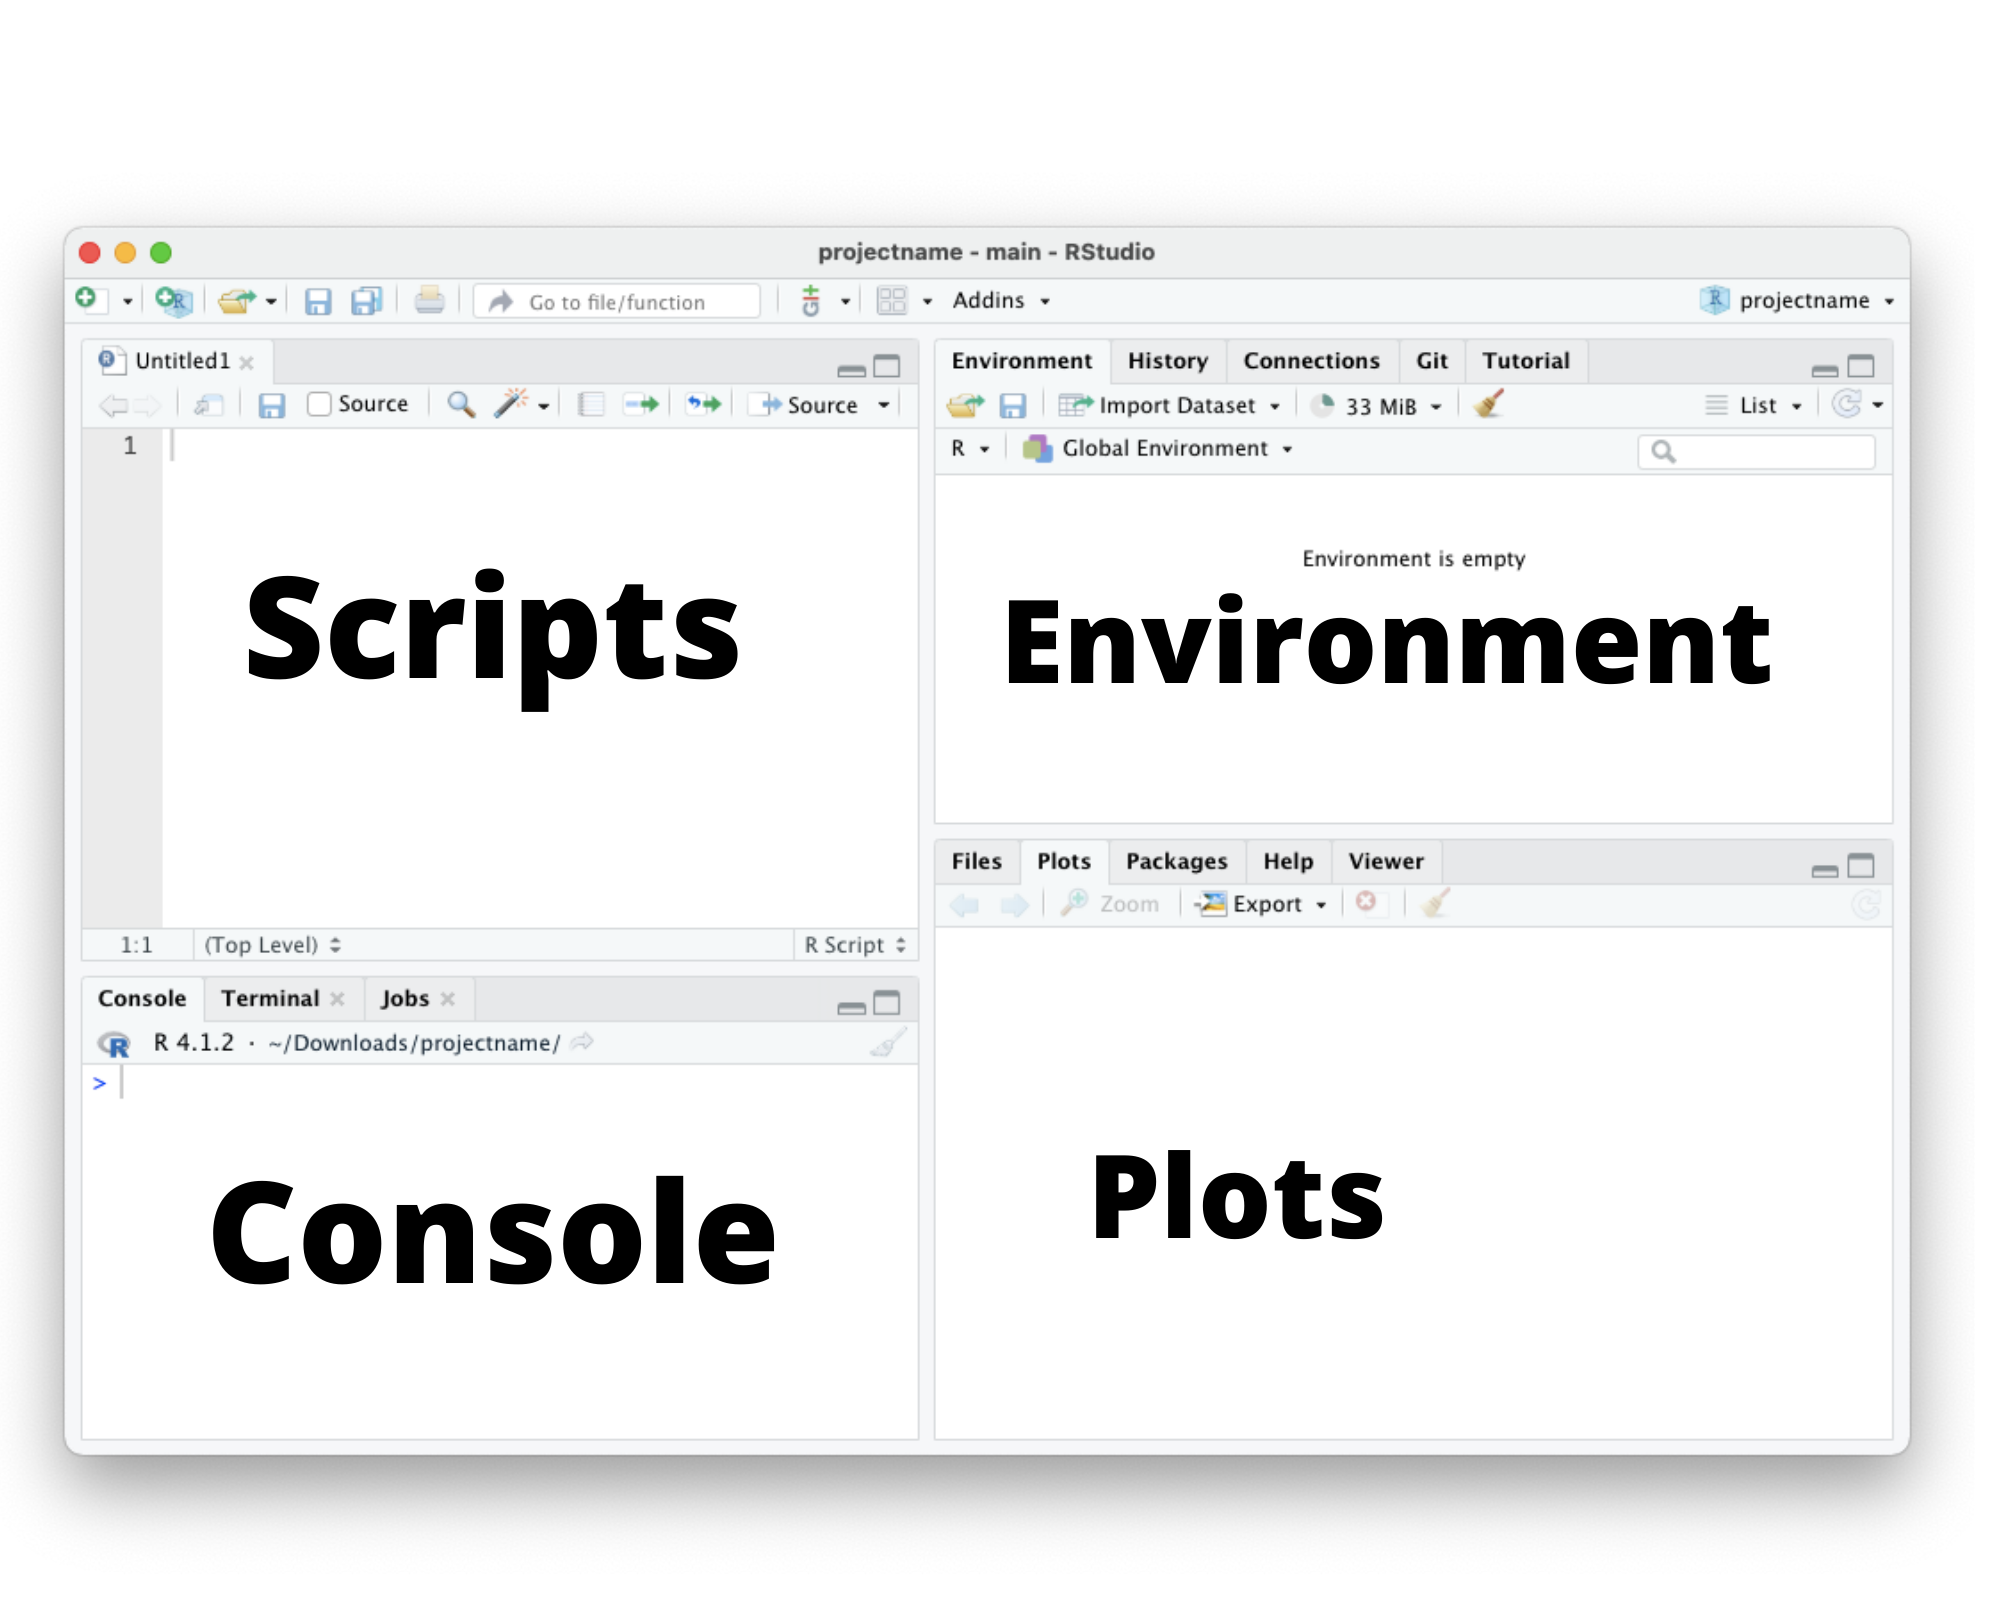
\includegraphics[width=3.125in,height=\textheight]{Console.png}\\
L'interface RStudio se présente ainsi par défaut. Nous pouvons voir une console, un environnement de travail, une partie pour les scripts et une autre pour la visualisation des graphiques.

\begin{itemize}
\tightlist
\item
  La \emph{console} peut servir à écrire une ligne d'instruction qui sera exécutée en appuyant sur Entrer.\\
\item
  La partie dédiée au \emph{scripts} permet d'écrire un ensemble de lignes de codes qui peuvent être exécutées par ordre voulu par l'utilisateur. En plus des scripts, on peut y visualiser nos tableaux de données qui sont décrits dans la section \ref{dataframe}.\\
\item
  Les graphes peuvent être visibles dans la partie \emph{Plots} de notre interface. Cette partie est un panneau contenant les onglets \emph{Viewer} pour les pages html, \emph{Files} pour naviguer dans les fichiers, \emph{Packages} pour gérer les packages installés et \emph{Help} pour chercher de l'aide.\\
\item
  La dernière partie c'est à dire \emph{Environment} est consacrée à la gestion de l'environnement de travail. Elle permet de voir les variables créés lors de notre session mais aussi d'avoir une idée sur leur structure
\end{itemize}

\hypertarget{firstcode}{%
\section{Premiers codes}\label{firstcode}}

Et si on écrivait notre premier code ?
Dans la section précédente nous avons présenté brièvement l'interface de RStudio, place maintenant à notre première instruction. Commencez par effectuer une petite opération d'addition (\texttt{2+3}) sur votre console puis appuyez sur Entrer.

\begin{Shaded}
\begin{Highlighting}[]
\DecValTok{2}\SpecialCharTok{+}\DecValTok{3}
\CommentTok{\#\textgreater{} [1] 5}
\end{Highlighting}
\end{Shaded}

Le résultat obtenu est tout naturellement \texttt{5}. Vous constatez que \texttt{{[}1{]}} précède le résultat de l'opération, en effet l'affichage se fait par défaut sous forme d'une liste\ref{list}.\\
La console peut être utilisée comme une calculatrice et supporte toutes les opérations arithmétiques telles que la soustraction(\texttt{-}), l'addition(\texttt{+}), la multiplication(\texttt{*}), la division décimale(\texttt{/}), la division entière(\texttt{\%/\%}), le modulo\footnote{modulo : Cet opérateur renvoi le reste de la division entre deux nombres} (\texttt{\%\%}).\\
Le symbole (\texttt{\#}) sert à écrire une ligne de commentaire.

\begin{Shaded}
\begin{Highlighting}[]
\DecValTok{1}\SpecialCharTok{+}\DecValTok{2} \CommentTok{\#addition}

\DecValTok{1{-}2} \CommentTok{\#Soustraction}

\DecValTok{1}\SpecialCharTok{/}\DecValTok{2} \CommentTok{\#Division decimale}

\DecValTok{1}\SpecialCharTok{\%/\%}\DecValTok{2} \CommentTok{\#Division entiere}

\DecValTok{1}\SpecialCharTok{\%\%}\DecValTok{2} \CommentTok{\#Modulo}
\end{Highlighting}
\end{Shaded}

On peut aussi effectuer des assignations sans déclarer les variables au préalable comme l'indique le code suivant.

\begin{Shaded}
\begin{Highlighting}[]
\NormalTok{x }\OtherTok{=} \DecValTok{1} \CommentTok{\#affection de la valeur 1 à x}
\NormalTok{y }\OtherTok{\textless{}{-}} \DecValTok{2} \CommentTok{\#affection de la valeur 2 à y}
\NormalTok{x}\SpecialCharTok{+}\NormalTok{y }\CommentTok{\#somme de x et y (1+2)}
\CommentTok{\#\textgreater{} [1] 3}
\end{Highlighting}
\end{Shaded}

\hypertarget{data-R}{%
\section{Données sur R}\label{data-R}}

Il existe 6 principaux types simples de données sur R sont : \emph{logical}, \emph{integer}, \emph{double}, \emph{complex}, \emph{character}, \emph{raw}.\\
Il arrive qu'une structure de données se compose de types simples données, c'est ce que nous allons étudier dans cette section.

\hypertarget{vecteur}{%
\subsection{Vecteur}\label{vecteur}}

\hypertarget{duxe9finition}{%
\subsubsection*{Définition}\label{duxe9finition}}
\addcontentsline{toc}{subsubsection}{Définition}

Le vecteur est un objet de base de R qui correspond à une liste d'éléments. Ses propriétés fondamentales sont :

\begin{itemize}
\tightlist
\item
  Dimension unitaire (les vecteurs sont unidimensionnel)\\
\item
  Éléments de même type (Toutes les valeurs contenues dans un vecteur sont de même type)\\
\item
  Longueur égale au nombre d'éléments
\end{itemize}

\hypertarget{cruxe9ation}{%
\subsubsection*{Création}\label{cruxe9ation}}
\addcontentsline{toc}{subsubsection}{Création}

La fonction la plus classique pour créer un vecteur est \texttt{c(...)}. Elle prend comme argument les éléments du vecteur. Dans le code suivant, nous allons créer un vecteur contenant les valeurs de 1 jusqu'à 5 puis nous allons le nommer \texttt{myvector}

\begin{Shaded}
\begin{Highlighting}[]
\NormalTok{myvector }\OtherTok{\textless{}{-}} \FunctionTok{c}\NormalTok{(}\DecValTok{1}\NormalTok{,}\DecValTok{2}\NormalTok{,}\DecValTok{3}\NormalTok{,}\DecValTok{4}\NormalTok{,}\DecValTok{5}\NormalTok{) }\CommentTok{\#Création}
\NormalTok{myvector }\CommentTok{\#Affichage}
\CommentTok{\#\textgreater{} [1] 1 2 3 4 5}
\end{Highlighting}
\end{Shaded}

Maintenant que nous avons un vecteur, il est naturel de se demander comment accéder aux éléments de ce dernier. Facile ! Il suffit de mettre entre crochet (\texttt{{[}{]}}), juste après le nom de votre vecteur, l'indice de l'élément voulu sachant que sur R le comptage commence par 1 au lieu de 0. Par exemple, dans la cellule suivante, le code permet d'afficher le quatrième élément c'est-à-dire celui qui a pour indice 4 de \texttt{myvector}.

\begin{Shaded}
\begin{Highlighting}[]
\NormalTok{myvector[}\DecValTok{4}\NormalTok{]}
\CommentTok{\#\textgreater{} [1] 4}
\end{Highlighting}
\end{Shaded}

Vous pouvez aussi supprimer un élément d'un vecteur en essayant de l'afficher avec l'opposé de son indice. Supprimons le premier élément de \texttt{myvector} !

\begin{Shaded}
\begin{Highlighting}[]
\NormalTok{myvector[}\SpecialCharTok{{-}}\DecValTok{1}\NormalTok{]}
\CommentTok{\#\textgreater{} [1] 2 3 4 5}
\end{Highlighting}
\end{Shaded}

Il se peut qu'on veuille créer une séquence de valeurs avec un pas spécifié. Un exemple concret c'est de vouloir créer un vecteur nommé \texttt{evenVector} contenant tous les nombres pairs compris entre 0 et 100. L'utilisation de la fonction \texttt{c()} rendrait le travail fastidieux. La fonction \texttt{seq()} est plus adaptée à notre situation. Elle prend comme argument from(le début de la séquence), to(la fin de la séquence), by(le pas de la séquence), etc. Pour en savoir plus vous pouvez exécuter la commande \texttt{?seq()}.

\begin{Shaded}
\begin{Highlighting}[]
\NormalTok{evenVector }\OtherTok{\textless{}{-}} \FunctionTok{seq}\NormalTok{(}\AttributeTok{from =} \DecValTok{0}\NormalTok{, }\AttributeTok{to =} \DecValTok{100}\NormalTok{, }\AttributeTok{by =} \DecValTok{2}\NormalTok{) }\CommentTok{\#Création }
\NormalTok{evenVector }\CommentTok{\#Affichage}
\CommentTok{\#\textgreater{}  [1]   0   2   4   6   8  10  12  14  16  18  20  22  24  26}
\CommentTok{\#\textgreater{} [15]  28  30  32  34  36  38  40  42  44  46  48  50  52  54}
\CommentTok{\#\textgreater{} [29]  56  58  60  62  64  66  68  70  72  74  76  78  80  82}
\CommentTok{\#\textgreater{} [43]  84  86  88  90  92  94  96  98 100}
\end{Highlighting}
\end{Shaded}

Si le pas de la séquence est de 1, on peut utiliser à la place de \texttt{seq()} l'opérateur \texttt{:} de premier terme le début de la séquence et de second terme la fin de la séquence. L'exemple qui suit permet de créer le vecteur \texttt{myvector} contenant tous les entiers de 1 à 5.

\begin{Shaded}
\begin{Highlighting}[]
\NormalTok{myvector }\OtherTok{\textless{}{-}} \DecValTok{1}\SpecialCharTok{:}\DecValTok{5}
\NormalTok{myvector}
\CommentTok{\#\textgreater{} [1] 1 2 3 4 5}
\end{Highlighting}
\end{Shaded}

Il est possible de créer un vecteur d'éléments répétitifs avec la fonction \texttt{rep()}. Supposons que nous voulons créer le vecteur \texttt{repvector} contenant 5 fois de suite tous les entiers de 1 à 10, nous allons donner en premier argument à la fonction \texttt{rep()} l'objet à répéter (\texttt{1:10}) et comme second argument le nombre de répétitions(\texttt{5}).

\begin{Shaded}
\begin{Highlighting}[]
\NormalTok{repvector }\OtherTok{\textless{}{-}} \FunctionTok{rep}\NormalTok{(}\DecValTok{1}\SpecialCharTok{:}\DecValTok{10}\NormalTok{,}\DecValTok{5}\NormalTok{)}
\NormalTok{repvector}
\CommentTok{\#\textgreater{}  [1]  1  2  3  4  5  6  7  8  9 10  1  2  3  4  5  6  7  8}
\CommentTok{\#\textgreater{} [19]  9 10  1  2  3  4  5  6  7  8  9 10  1  2  3  4  5  6}
\CommentTok{\#\textgreater{} [37]  7  8  9 10  1  2  3  4  5  6  7  8  9 10}
\end{Highlighting}
\end{Shaded}

\hypertarget{facteur}{%
\subsection{Facteur}\label{facteur}}

\hypertarget{duxe9finition-1}{%
\subsubsection*{Définition}\label{duxe9finition-1}}
\addcontentsline{toc}{subsubsection}{Définition}

Le facteur (\emph{factor}) est un vecteur de valeurs d'une variable catégorielle. Très souvevent, les variables qualitatives sont catégorielles c'est le cas du sexe(Homme, Femme), des questions directes(Oui, Non), etc.C'est d'ailleurs la raison de l'existance de cet objet sur R qui est très utiles dans certaines representations graphiques.Le caractère principal de \emph{factor} est qu'il dispose de niveaux appelés \texttt{levels}. Ces derniers sont uniques et peuvent avoir des valeurs qui ne sont pas contenus par le facteur.

\hypertarget{cruxe9ation-1}{%
\subsubsection*{Création}\label{cruxe9ation-1}}
\addcontentsline{toc}{subsubsection}{Création}

Pour créer un facteur, on commence par créer un vecteur puis avec la fonction \texttt{factor()} nous pouvons le transformer en objet de type facteur. Par défaut, les niveaux des facteurs sont les modalités prises par le vecteur. Pour modifier les niveaux on utilise l'argument \texttt{levels} de la fonction \texttt{factor()} pour spécifier notre vecteur de niveaux.
On se propose de transformer en facteur le vecteur \texttt{animal} de modalités \emph{chat}, \emph{souris}, \emph{chien} en un facteur de niveaux \emph{chat}, \emph{souris}, \emph{chien} et \emph{rat}.

\begin{Shaded}
\begin{Highlighting}[]
\NormalTok{animal }\OtherTok{\textless{}{-}} \FunctionTok{c}\NormalTok{(}\StringTok{"souris"}\NormalTok{,}\StringTok{"souris"}\NormalTok{,}\StringTok{"chien"}\NormalTok{,}\StringTok{"chat"}\NormalTok{,}\StringTok{"chien"}\NormalTok{,}\StringTok{"chat"}\NormalTok{,}\StringTok{"souris"}\NormalTok{,}\StringTok{"chat"}\NormalTok{,}\StringTok{"chat"}\NormalTok{,}\StringTok{"chien"}\NormalTok{)}
\NormalTok{myfactor }\OtherTok{\textless{}{-}} \FunctionTok{factor}\NormalTok{(animal,}\AttributeTok{levels =} \FunctionTok{c}\NormalTok{(}\StringTok{\textquotesingle{}chat\textquotesingle{}}\NormalTok{,}\StringTok{\textquotesingle{}souris\textquotesingle{}}\NormalTok{,}\StringTok{\textquotesingle{}chien\textquotesingle{}}\NormalTok{,}\StringTok{\textquotesingle{}rat\textquotesingle{}}\NormalTok{))}
\NormalTok{myfactor}
\CommentTok{\#\textgreater{}  [1] souris souris chien  chat   chien  chat   souris chat  }
\CommentTok{\#\textgreater{}  [9] chat   chien }
\CommentTok{\#\textgreater{} Levels: chat souris chien rat}
\end{Highlighting}
\end{Shaded}

\hypertarget{list}{%
\subsection{Liste}\label{list}}

\hypertarget{duxe9finition-2}{%
\subsubsection*{Définition}\label{duxe9finition-2}}
\addcontentsline{toc}{subsubsection}{Définition}

Une liste est un objet pouvant contenir des éléments de tous types. L'homogénéité du type des éléments n'est pas obligatoire dans une liste c'est à dire qu'elle peut contenir des listes, des vecteurs, des matrices, des fonctions etc. On peut nommer les éléments d'une liste lors de sa création en effectuant des affections.

\hypertarget{cruxe9ation-2}{%
\subsubsection*{Création}\label{cruxe9ation-2}}
\addcontentsline{toc}{subsubsection}{Création}

La création d'une liste se fait avec la fonction \texttt{list()} qui prend en argument les éléments à concaténer.

\begin{Shaded}
\begin{Highlighting}[]
\NormalTok{mylist }\OtherTok{=} \FunctionTok{list}\NormalTok{(}\AttributeTok{num =} \FunctionTok{c}\NormalTok{(}\DecValTok{1}\NormalTok{,}\DecValTok{2}\NormalTok{,}\DecValTok{3}\NormalTok{), }\AttributeTok{char =} \StringTok{\textquotesingle{}character\textquotesingle{}}\NormalTok{)}
\NormalTok{mylist}
\CommentTok{\#\textgreater{} $num}
\CommentTok{\#\textgreater{} [1] 1 2 3}
\CommentTok{\#\textgreater{} }
\CommentTok{\#\textgreater{} $char}
\CommentTok{\#\textgreater{} [1] "character"}
\end{Highlighting}
\end{Shaded}

On peut accéder à un élément par son nom en utilisant le symbole \texttt{\$} (\texttt{malist\$nomElement}). L'accès à l'élément \texttt{num} de \texttt{mylist} peut se faire de la manière suivante :

\begin{Shaded}
\begin{Highlighting}[]
\NormalTok{mylist}\SpecialCharTok{$}\NormalTok{num}
\CommentTok{\#\textgreater{} [1] 1 2 3}
\end{Highlighting}
\end{Shaded}

Un autre moyen d'accéder à un élément d'une liste c'est par son indice mis entre deux crochets (\texttt{{[}{[}index{]}{]}}) juste après le nom de la liste. On peut reprendre l'accès à l'élément \texttt{num} par indexation.

\begin{Shaded}
\begin{Highlighting}[]
\NormalTok{mylist[[}\DecValTok{1}\NormalTok{]]}
\CommentTok{\#\textgreater{} [1] 1 2 3}
\end{Highlighting}
\end{Shaded}

On peut modifier l'élément \texttt{num} de mylist en lui affectant une nouvelle valeur.

\begin{Shaded}
\begin{Highlighting}[]
\NormalTok{mylist}\SpecialCharTok{$}\NormalTok{num }\OtherTok{=} \DecValTok{1}\SpecialCharTok{:}\DecValTok{10}
\NormalTok{mylist}\SpecialCharTok{$}\NormalTok{num}
\CommentTok{\#\textgreater{}  [1]  1  2  3  4  5  6  7  8  9 10}
\end{Highlighting}
\end{Shaded}

L'ajout d'un nouvel élément dans \texttt{mylist} peut aussi se faire facilement. Si on se propose d'ajouter un élément nommé \texttt{logical} qui reçoit initialement \texttt{TRUE} on peut procéder ainsi :

\begin{Shaded}
\begin{Highlighting}[]
\NormalTok{mylist}\SpecialCharTok{$}\NormalTok{logical }\OtherTok{=} \ConstantTok{TRUE}
\NormalTok{mylist}
\CommentTok{\#\textgreater{} $num}
\CommentTok{\#\textgreater{}  [1]  1  2  3  4  5  6  7  8  9 10}
\CommentTok{\#\textgreater{} }
\CommentTok{\#\textgreater{} $char}
\CommentTok{\#\textgreater{} [1] "character"}
\CommentTok{\#\textgreater{} }
\CommentTok{\#\textgreater{} $logical}
\CommentTok{\#\textgreater{} [1] TRUE}
\end{Highlighting}
\end{Shaded}

\hypertarget{matrice}{%
\subsection{Matrice}\label{matrice}}

\hypertarget{duxe9finition-3}{%
\subsubsection*{Définition}\label{duxe9finition-3}}
\addcontentsline{toc}{subsubsection}{Définition}

Une matrice est un un tableau dont les colonnes sont des vecteurs de même type et de même taille. Autrement dit, la matrice est un objet de deux dimensions dont tous les éléments sont de type homogène. R ne considère pas un vecteur comme une matrice colonne ou ligne, ce sont deux types de structures différentes.

\hypertarget{cruxe9ation-3}{%
\subsubsection*{Création}\label{cruxe9ation-3}}
\addcontentsline{toc}{subsubsection}{Création}

Une matrice colonne se crée avec la fonction \texttt{cbind()} et la matrice ligne par \texttt{rbind()}. Pour créer une matrice de plusieurs colonnes on utilise la fonction \texttt{matrix()}.
Vous pouvez avoir une documentation complète de ces fonctions en exécutant la commande faisant précéder d'un point d'interrogation le nom de votre fonction ( \emph{Exemple} : \texttt{?cbind()}) dans votre console.

\begin{Shaded}
\begin{Highlighting}[]
\CommentTok{\#matrice colonne}
\NormalTok{colMatrix }\OtherTok{\textless{}{-}} \FunctionTok{cbind}\NormalTok{(}\DecValTok{1}\SpecialCharTok{:}\DecValTok{5}\NormalTok{)}
\NormalTok{colMatrix}
\CommentTok{\#\textgreater{}      [,1]}
\CommentTok{\#\textgreater{} [1,]    1}
\CommentTok{\#\textgreater{} [2,]    2}
\CommentTok{\#\textgreater{} [3,]    3}
\CommentTok{\#\textgreater{} [4,]    4}
\CommentTok{\#\textgreater{} [5,]    5}
\end{Highlighting}
\end{Shaded}

\begin{Shaded}
\begin{Highlighting}[]
\CommentTok{\#matrice ligne}
\NormalTok{rowMatrix }\OtherTok{\textless{}{-}} \FunctionTok{rbind}\NormalTok{(}\DecValTok{1}\SpecialCharTok{:}\DecValTok{5}\NormalTok{)}
\NormalTok{rowMatrix}
\CommentTok{\#\textgreater{}      [,1] [,2] [,3] [,4] [,5]}
\CommentTok{\#\textgreater{} [1,]    1    2    3    4    5}
\end{Highlighting}
\end{Shaded}

\begin{Shaded}
\begin{Highlighting}[]
\CommentTok{\#matrice}
\NormalTok{Matrix }\OtherTok{\textless{}{-}} \FunctionTok{matrix}\NormalTok{(}\FunctionTok{c}\NormalTok{(}\AttributeTok{x=}\NormalTok{ (}\DecValTok{1}\SpecialCharTok{:}\DecValTok{5}\NormalTok{), }\AttributeTok{y =} \FunctionTok{rep}\NormalTok{(}\DecValTok{1}\NormalTok{,}\DecValTok{5}\NormalTok{)),}\AttributeTok{nrow =} \DecValTok{5}\NormalTok{)}
\NormalTok{Matrix}
\CommentTok{\#\textgreater{}      [,1] [,2]}
\CommentTok{\#\textgreater{} [1,]    1    1}
\CommentTok{\#\textgreater{} [2,]    2    1}
\CommentTok{\#\textgreater{} [3,]    3    1}
\CommentTok{\#\textgreater{} [4,]    4    1}
\CommentTok{\#\textgreater{} [5,]    5    1}
\end{Highlighting}
\end{Shaded}

On peut accéder aux éléments de la matrice par leurs indices. Comme on le fait en maths, il faut d'abord mettre le numéro de la ligne puis le numéro de la colonne séparée par une virgule.
On peut afficher une ligne (respectivement une colonne )toute entière en spécifiant seulement l'indice de la ligne (respectivement la colonne).

\begin{Shaded}
\begin{Highlighting}[]
\CommentTok{\# Accès à l\textquotesingle{}élément de la ligne 4 et de la colonne 1}
\NormalTok{Matrix[}\DecValTok{4}\NormalTok{,}\DecValTok{1}\NormalTok{]}
\CommentTok{\#\textgreater{} [1] 4}
\end{Highlighting}
\end{Shaded}

\begin{Shaded}
\begin{Highlighting}[]
\CommentTok{\# Accès à  la ligne 2 }
\NormalTok{Matrix[}\DecValTok{2}\NormalTok{,]}
\CommentTok{\#\textgreater{} [1] 2 1}
\end{Highlighting}
\end{Shaded}

\begin{Shaded}
\begin{Highlighting}[]
\CommentTok{\# Accès à la colonne 3}
\NormalTok{Matrix[,}\DecValTok{2}\NormalTok{]}
\CommentTok{\#\textgreater{} [1] 1 1 1 1 1}
\end{Highlighting}
\end{Shaded}

\hypertarget{dataframe}{%
\subsection{Tableau de données ou Data frame}\label{dataframe}}

\hypertarget{duxe9finition-4}{%
\subsubsection*{Définition}\label{duxe9finition-4}}
\addcontentsline{toc}{subsubsection}{Définition}

Un tableau de données (data frame) est comme la matrice, un objet de deux dimensions sauf qu'il peut contenir des colonnes de types différents. Chaque colonne doit contenir des éléments de même type. La data.frame est un objet très utilisé sur R et ce sera le cas dans les chapitres suivants de ce livre.

\hypertarget{cruxe9ation-4}{%
\subsubsection*{Création}\label{cruxe9ation-4}}
\addcontentsline{toc}{subsubsection}{Création}

La fonction \texttt{data.frame()} permet de créer un tableau de données. Elle prend en argument des vecteurs de même longueur. Il en existe d'autres arguments pour cette fonction, pour en savoir plus vous pouvez exécuter \texttt{?data.frame()}.

\begin{Shaded}
\begin{Highlighting}[]
\NormalTok{x }\OtherTok{=} \FunctionTok{c}\NormalTok{(}\DecValTok{12}\NormalTok{,}\DecValTok{67}\NormalTok{,}\DecValTok{13}\NormalTok{)}
\NormalTok{y }\OtherTok{=} \FunctionTok{c}\NormalTok{(}\StringTok{\textquotesingle{}A\textquotesingle{}}\NormalTok{,}\StringTok{\textquotesingle{}B\textquotesingle{}}\NormalTok{,}\StringTok{\textquotesingle{}C\textquotesingle{}}\NormalTok{)}
\NormalTok{tableau }\OtherTok{=} \FunctionTok{data.frame}\NormalTok{(x,y)}
\NormalTok{tableau}
\CommentTok{\#\textgreater{}    x y}
\CommentTok{\#\textgreater{} 1 12 A}
\CommentTok{\#\textgreater{} 2 67 B}
\CommentTok{\#\textgreater{} 3 13 C}
\end{Highlighting}
\end{Shaded}

L'accès à un élément peut se faire de la même manière qu'avec les matrices. Pour accéder à une colonne par son nom on utilise le symbole comme dans la section liste. Les codes suivants permettent d'accéder à l'élément ``B'' du \texttt{tableau} de plusieurs façons.

\begin{Shaded}
\begin{Highlighting}[]
\CommentTok{\#Indexiation}
\NormalTok{tableau[}\DecValTok{2}\NormalTok{,}\DecValTok{2}\NormalTok{]}
\CommentTok{\#\textgreater{} [1] "B"}
\end{Highlighting}
\end{Shaded}

\begin{Shaded}
\begin{Highlighting}[]
\CommentTok{\#Par le nom de la colonne}
\NormalTok{tableau}\SpecialCharTok{$}\NormalTok{y[}\DecValTok{2}\NormalTok{]}
\CommentTok{\#\textgreater{} [1] "B"}
\end{Highlighting}
\end{Shaded}

\begin{Shaded}
\begin{Highlighting}[]
\NormalTok{tableau[[}\StringTok{\textquotesingle{}y\textquotesingle{}}\NormalTok{]][}\DecValTok{2}\NormalTok{]}
\CommentTok{\#\textgreater{} [1] "B"}
\end{Highlighting}
\end{Shaded}

\hypertarget{les-boucles-et-conditions}{%
\section{Les boucles et conditions}\label{les-boucles-et-conditions}}

\hypertarget{les-boucles}{%
\subsection{Les boucles}\label{les-boucles}}

Les boucles permettent de gérer des instructions répétitives. Sur R il est plus pratique d'utiliser la vectorisation, mais pour débuter, les boucles feront l'affaire.

\hypertarget{for}{%
\subsubsection*{for}\label{for}}
\addcontentsline{toc}{subsubsection}{for}

La boucle for permet d'itérer sur un vecteur de longueur connu d'avance. La syntaxe est la suivante :

\begin{Shaded}
\begin{Highlighting}[]
\ControlFlowTok{for}\NormalTok{ (variable }\ControlFlowTok{in}\NormalTok{ vector) \{}
\NormalTok{  statements}
\NormalTok{\}}
\end{Highlighting}
\end{Shaded}

Un exemple de création d'un vecteur de 5 éléments contenant les carrés des nombre compris entre 1 et 5

\begin{Shaded}
\begin{Highlighting}[]
\CommentTok{\#Initialisation}
\NormalTok{carrevector }\OtherTok{=} \DecValTok{0}
\CommentTok{\#Boucle}
\ControlFlowTok{for}\NormalTok{ (i }\ControlFlowTok{in} \DecValTok{1}\SpecialCharTok{:}\DecValTok{5}\NormalTok{) \{}
\NormalTok{  carrevector[i]}\OtherTok{=}\NormalTok{i}\SpecialCharTok{\^{}}\DecValTok{2}
\NormalTok{\}}
\CommentTok{\#affichage}
\NormalTok{carrevector}
\CommentTok{\#\textgreater{} [1]  1  4  9 16 25}
\end{Highlighting}
\end{Shaded}

\hypertarget{while}{%
\subsubsection*{While}\label{while}}
\addcontentsline{toc}{subsubsection}{While}

Si le nombre d'itérations n'est pas connu d'avance alors que la condition d'arrêt si, il est préférable d'utiliser la boucle while. Elle permet de répéter une instruction tant qu'une condition est satisfaite. la syntaxe est la suivante :

\begin{Shaded}
\begin{Highlighting}[]
\ControlFlowTok{while}\NormalTok{ (condition) \{}
\NormalTok{  statements}
\NormalTok{\}}
\end{Highlighting}
\end{Shaded}

Avec la boucle while on peut chercher le premier élément supérieur à 10 dans \texttt{carrevector}. Les deux conditions d'arrêts sont alors : l'élément(\texttt{x}) supérieur à 10 et(\texttt{\&}) l'indice(\texttt{j}) supérieur à la longueur du vecteur(\texttt{5}).

\begin{Shaded}
\begin{Highlighting}[]
\CommentTok{\# Initialisation}
\NormalTok{j }\OtherTok{=} \DecValTok{1}
\CommentTok{\# Boucle}
\ControlFlowTok{while}\NormalTok{ (carrevector[j]}\SpecialCharTok{\textless{}=}\DecValTok{10} \SpecialCharTok{\&}\NormalTok{ j}\SpecialCharTok{\textless{}=} \DecValTok{5}\NormalTok{)\{}
\NormalTok{  j}\OtherTok{=}\NormalTok{j}\SpecialCharTok{+}\DecValTok{1}
\NormalTok{\}}
\NormalTok{x}\OtherTok{=}\NormalTok{carrevector[j]}
\CommentTok{\# Affichage}
\NormalTok{x}
\CommentTok{\#\textgreater{} [1] 16}
\end{Highlighting}
\end{Shaded}

\hypertarget{les-conditions}{%
\subsection{Les conditions}\label{les-conditions}}

Elles permettent d'exécuter des instructions si une ou des conditions sont satisfaites. la syntaxe la plus simple est :

\begin{Shaded}
\begin{Highlighting}[]
\ControlFlowTok{if}\NormalTok{ (condition) \{}
  \CommentTok{\#statements}
\NormalTok{\}}\ControlFlowTok{else}\NormalTok{\{}
  \CommentTok{\#statements}
\NormalTok{\}}
\end{Highlighting}
\end{Shaded}

\textbf{Exemple} :

\begin{Shaded}
\begin{Highlighting}[]
\NormalTok{num }\OtherTok{=} \DecValTok{10}
\ControlFlowTok{if}\NormalTok{ (num }\SpecialCharTok{\textgreater{}} \DecValTok{0}\NormalTok{) \{}
  \FunctionTok{print}\NormalTok{(}\StringTok{\textquotesingle{}Ce nombre est positif\textquotesingle{}}\NormalTok{)}
\NormalTok{\}}\ControlFlowTok{else}\NormalTok{\{}
  \FunctionTok{print}\NormalTok{(}\StringTok{\textquotesingle{}Ce nombre est negatif\textquotesingle{}}\NormalTok{)}
\NormalTok{\}}
\CommentTok{\#\textgreater{} [1] "Ce nombre est positif"}
\end{Highlighting}
\end{Shaded}

\hypertarget{les-fonctions}{%
\section{Les fonctions}\label{les-fonctions}}

Si dans un projet vous aurez à utiliser plusieurs fois un bloc d'instructions, l'idéal c'est de créer des fonctions. Pour cela, on a besoin de \texttt{function()} que l'on assigne au nom de notre fonction.
Les fonctions peuvent retourner une valeur ou bien exécuter seulement un ensemble d'instructions.

\begin{Shaded}
\begin{Highlighting}[]
\NormalTok{mafonction  }\OtherTok{\textless{}{-}} \ControlFlowTok{function}\NormalTok{(arguments) \{}
\NormalTok{  instructions}
  \FunctionTok{return}\NormalTok{(valuer)}
\NormalTok{\}}
\end{Highlighting}
\end{Shaded}

Pour créer la fonction \texttt{addition} qui somme deux éléments \texttt{x} et \texttt{y} on procède ainsi :

\begin{Shaded}
\begin{Highlighting}[]
\NormalTok{addition }\OtherTok{\textless{}{-}} \ControlFlowTok{function}\NormalTok{(x,y)\{}
  \FunctionTok{return}\NormalTok{(x}\SpecialCharTok{+}\NormalTok{y)}
\NormalTok{\}}
\CommentTok{\#Ou bien}
\NormalTok{addition }\OtherTok{\textless{}{-}} \ControlFlowTok{function}\NormalTok{(x,y)\{}
\NormalTok{  x}\SpecialCharTok{+}\NormalTok{y}
\NormalTok{\}}
\end{Highlighting}
\end{Shaded}

Pour utiliser la fonction il suffit de l'appeler en indiquant les valeurs de ses arguments entre parenthèses.

\begin{Shaded}
\begin{Highlighting}[]
\CommentTok{\# somme de 10 et de 4}
\FunctionTok{addition}\NormalTok{(}\DecValTok{10}\NormalTok{,}\DecValTok{4}\NormalTok{)}
\CommentTok{\#\textgreater{} [1] 14}
\end{Highlighting}
\end{Shaded}

\hypertarget{liens-utils}{%
\section*{Liens utils}\label{liens-utils}}
\addcontentsline{toc}{section}{Liens utils}

\citet{base}\strut \\
\url{https://cran.r-project.org/doc/contrib/Paradis-rdebuts_fr.pdf}

\hypertarget{part-ii-regressions}{%
\part{II-Regressions}\label{part-ii-regressions}}

\hypertarget{simple-lm}{%
\chapter{La régression linéaire simple}\label{simple-lm}}

\hypertarget{introduction}{%
\section{Introduction}\label{introduction}}

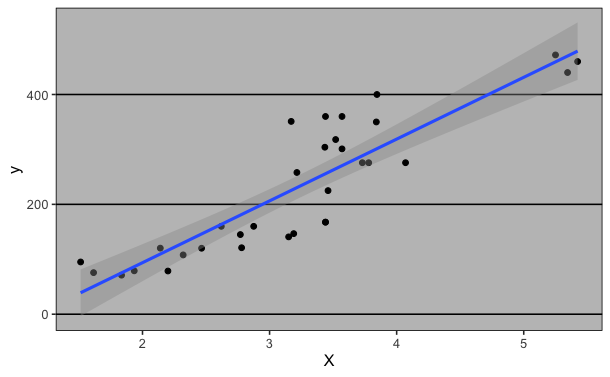
\includegraphics[width=3.125in,height=\textheight]{Pictures/lm.png} La régression linéaire
simple est une méthode statistique permettant de trouver une relation
linéaire entre une variable explicative \(X\) et une variable à expliquer
\(y\). Ce modèle consiste à considérer \(y\) comme une fonction affine de
\(X\). En d'autre terme, la régression linéaire a pour but de trouver une
droite ajustée au nuage de points de \(y\) en fonction de \(X\).\\
Dans ce chapitres nous allons voir en détail le modèle linéaire simple
ainsi que son application avec R. Nous utiliserons les données de
\href{https://github.com/AODiakite/r4econometrics/blob/master/Data/income.data.csv}{income}
disponible sur github. Vous pouvez télécharger le jeux de données avec
la fonction \texttt{read\_csv()} disponible dans le package \texttt{readr} comme suit :

\begin{Shaded}
\begin{Highlighting}[]
\FunctionTok{library}\NormalTok{(readr)}
\NormalTok{income }\OtherTok{=} \FunctionTok{read\_csv}\NormalTok{(}\StringTok{"https://github.com/AODiakite/r4econometrics/blob/master/Data/income.data.csv"}\NormalTok{)}
\end{Highlighting}
\end{Shaded}

\begin{table}

\caption{\label{tab:unnamed-chunk-3}Données pour la régression linéaire simple : income( niveau de revenu par 10 000 dollars ), happiness(score du bonheur entre 0 et 10), nombre d’observations(498)}
\centering
\begin{tabular}[t]{rr}
\toprule
income & happiness\\
\midrule
3.862647 & 2.314489\\
4.979381 & 3.433490\\
4.923957 & 4.599373\\
3.214372 & 2.791114\\
7.196409 & 5.596398\\
\addlinespace
3.729643 & 2.458556\\
4.674517 & 3.192992\\
4.498104 & 1.907137\\
3.121631 & 2.942450\\
4.639914 & 3.737942\\
\bottomrule
\end{tabular}
\end{table}

\hypertarget{moduxe9lisation-mathuxe9matique}{%
\section{Modélisation mathématique}\label{moduxe9lisation-mathuxe9matique}}

L'ajustement affine de \(y\) par \(X\) stipule que que y peut s'écrire comme
équation d'une droite :

\begin{equation}
y = \beta_0 + \beta_1 X  
\label{eq:lm}
\end{equation}

\begin{itemize}
\tightlist
\item
  \(y(y_1,y_2,\dots,y_n)\) : variable à expliquer, variable dépendante,
  variable endogène, variable réponse\\
\item
  \(X(x_1,x_2,\dots,x_n)\) : variable explicative,variable exogène,
  Variable régresseur\\
\item
  \(\beta_0\) : l'ordonnée à l'origine, coefficient inconnu
\item
  \(\beta_1\) : la pente de la droite, coefficient inconnu
\end{itemize}

En réalité sauf dans le cas d'un modèle parfait, la liaison linéaire
\eqref{eq:lm} entre y et X est perturbée par un bruit \(\epsilon\).
l'équation du modèle devient alors :

\begin{equation}
y = \beta_0 + \beta_1 X +\epsilon
\label{eq:lm-simple}
\end{equation}

La variable aléatoire \(\epsilon\) est indépendante de \(X\) et est supposée
suivre une loi normale de moyenne \(0\) et d'écart type \(\sigma\) :

\[ (\epsilon_1,\epsilon_2,\dots,\epsilon_n)= \epsilon \sim \mathcal{N}(0,\,\sigma^{2})\]

Pour le jeu de données \texttt{income} nous allons prendre comme variable
exogène \(X\) les revenus des individus(\texttt{income}) et le niveau de
bonheur(\texttt{happiness}) comme variable endogène \(y\). Ce choix n'est pas
hasardeux, car dans la régression linéaire, la variable indépendante
doit être déterministe c'est à un dire ne comportant pas de caractère
aléatoire alors que la variable dépendante comporte quant à elle un
bruit aléatoire \(\epsilon\).\\
Du fait que la moyenne de \(\epsilon\) soit nulle, l'équation
\eqref{eq:lm-simple} revient juste à une estimation d'une moyenne
conditionnelle :

\begin{equation}
\mathbb{E}(y_i|X_i) = \beta_0 + \beta_1 X_i
\label{eq:lm-E}
\end{equation}

La première étape lors d'une régression linéaire c'est la représentation
graphique du nuage de points. En effet si le nuage ne s'apparente pas à
une droite, la régression linéaire ne sera pas le meilleur modèle pour
notre jeu de données. Dans cet ouvrage nous utiliserons le package
ggplot2\footnote{ggplot2 :
  \url{https://r4ds.had.co.nz/data-visualisation.html}} pour nos représentations graphiques.

\begin{Shaded}
\begin{Highlighting}[]
\FunctionTok{library}\NormalTok{(ggplot2) }\CommentTok{\#Chargement du package}
\NormalTok{fig1 }\OtherTok{=} \FunctionTok{ggplot}\NormalTok{(}\AttributeTok{data =}\NormalTok{ income,}\FunctionTok{aes}\NormalTok{(}\AttributeTok{x =}\NormalTok{income, }\AttributeTok{y =}\NormalTok{ happiness)) }\SpecialCharTok{+}
               \FunctionTok{geom\_point}\NormalTok{()}
\NormalTok{fig1}
\end{Highlighting}
\end{Shaded}

\begin{figure}

{\centering 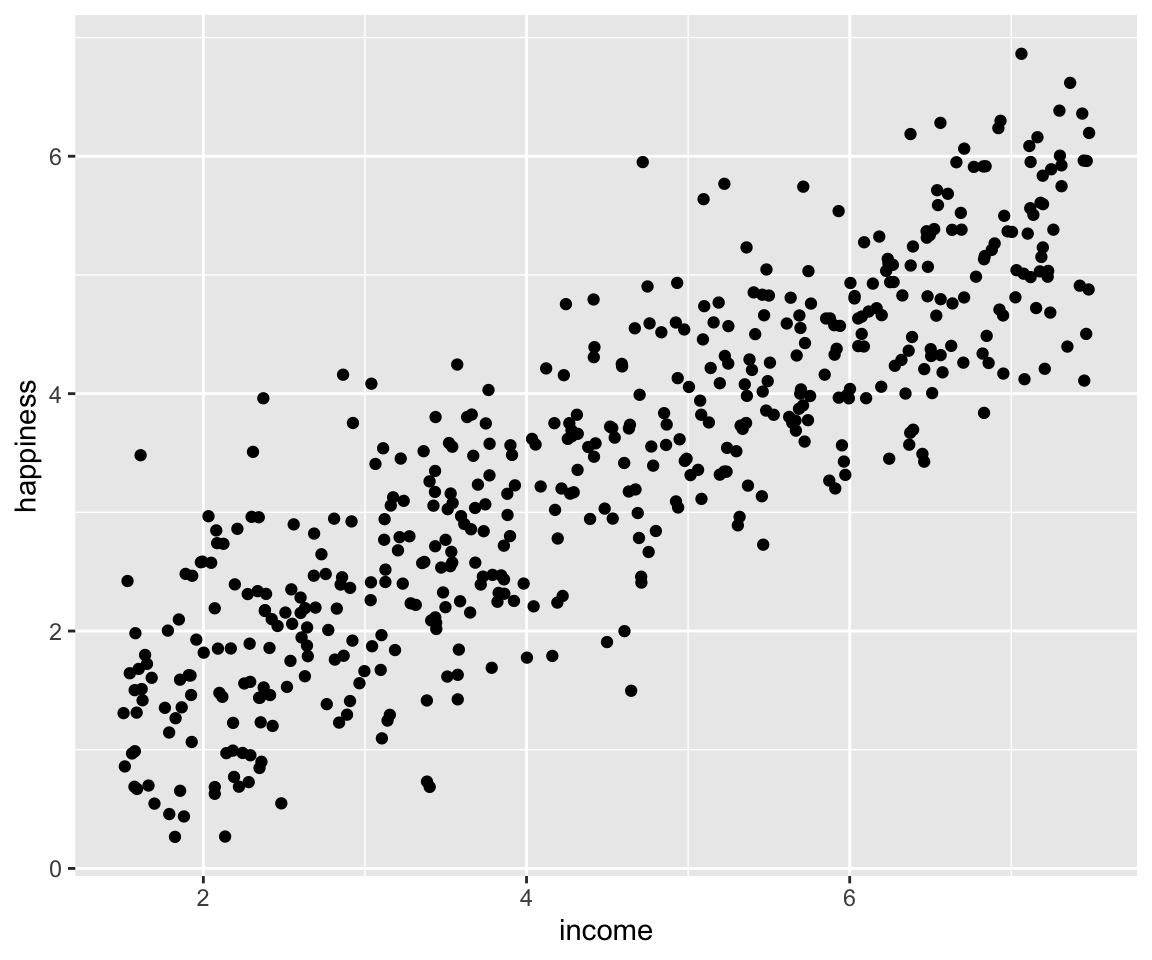
\includegraphics{03-simple-lm_files/figure-latex/nuage1-1} 

}

\caption{A première vue, ce nuage admet bien une tendance linéaire.}\label{fig:nuage1}
\end{figure}

\hypertarget{OLS}{%
\section{\texorpdfstring{Estimateurs des moindres carrés ordinaires (\(MCO\))}{Estimateurs des moindres carrés ordinaires (MCO)}}\label{OLS}}

La problématique du modèle\eqref{eq:lm-simple}, c'est de trouver les
coefficients \(\beta_i\) qui donnent un meilleur ajustement linéaire de
\(y\). Pour cela on a recours aux estimateurs des moindres qui carrés.
Cette méthode consiste à trouver les coefficients qui minimise la
quantité :

\begin{equation}

(\beta_0,\beta_1) = \sum\limits^{n}_{i=1}(y_i -\beta_0-\beta_1 x_i)^2=\sum\limits^{n}_{i=1}\epsilon_i^2
\label{eq:OLS}

\end{equation}

Les estimateurs \(\hat{\beta}_i\) s'écrivent donc de la forme :

\[(\hat\beta_0,\hat\beta_1) =\operatorname*{argmin}_{(\beta_0,\beta_1)\in \mathbb{R}\times\mathbb{R}}S(\beta_0,\beta_1)\]

La fonction \(S\) est strictement convexe donc si elle admet un point
singulier, celui-ci correspondra à l'unique minimum. Les estimateurs des
moindres carrés sont obtenus en résolvant le système d'équation qui
annule les dérivées partielles de \(S\) aux points \(\beta_i\). Le résultat
de ce système est :

\[\hat{\beta}_1 = \frac{\sum(x_i – \bar{x}) (y_i – \bar{y})} {\sum(x_i – \bar{x})^2} = \frac{Cov(X,y)}{Var(X)}\]
\[\hat{\beta}_0 = \bar{y} – \hat{\beta}_1 \bar{x}\]
\[avec\; :\; \bar{y} = \frac{1}{n}\sum\limits_{i=1}^n y_i\; et\; \bar{x} = \frac{1}{n}\sum\limits_{i=1}^n x_i \]

La fonction \texttt{lm()} permet d'entrainer un modèle linéaire sur R. Dans
notre exemple, on procède ainsi :

\begin{Shaded}
\begin{Highlighting}[]
\NormalTok{lm\_simple }\OtherTok{\textless{}{-}} \FunctionTok{lm}\NormalTok{(}\AttributeTok{formula =}\NormalTok{ happiness}\SpecialCharTok{\textasciitilde{}}\NormalTok{income, }\AttributeTok{data =}\NormalTok{ income)}
\end{Highlighting}
\end{Shaded}

\begin{Shaded}
\begin{Highlighting}[]
\FunctionTok{summary}\NormalTok{(lm\_simple)}
\CommentTok{\#\textgreater{} }
\CommentTok{\#\textgreater{} Call:}
\CommentTok{\#\textgreater{} lm(formula = happiness \textasciitilde{} income, data = income)}
\CommentTok{\#\textgreater{} }
\CommentTok{\#\textgreater{} Residuals:}
\CommentTok{\#\textgreater{}      Min       1Q   Median       3Q      Max }
\CommentTok{\#\textgreater{} {-}2.02479 {-}0.48526  0.04078  0.45898  2.37805 }
\CommentTok{\#\textgreater{} }
\CommentTok{\#\textgreater{} Coefficients:}
\CommentTok{\#\textgreater{}             Estimate Std. Error t value Pr(\textgreater{}|t|)    }
\CommentTok{\#\textgreater{} (Intercept)  0.20427    0.08884   2.299   0.0219 *  }
\CommentTok{\#\textgreater{} income       0.71383    0.01854  38.505   \textless{}2e{-}16 ***}
\CommentTok{\#\textgreater{} {-}{-}{-}}
\CommentTok{\#\textgreater{} Signif. codes:  }
\CommentTok{\#\textgreater{} 0 \textquotesingle{}***\textquotesingle{} 0.001 \textquotesingle{}**\textquotesingle{} 0.01 \textquotesingle{}*\textquotesingle{} 0.05 \textquotesingle{}.\textquotesingle{} 0.1 \textquotesingle{} \textquotesingle{} 1}
\CommentTok{\#\textgreater{} }
\CommentTok{\#\textgreater{} Residual standard error: 0.7181 on 496 degrees of freedom}
\CommentTok{\#\textgreater{} Multiple R{-}squared:  0.7493, Adjusted R{-}squared:  0.7488 }
\CommentTok{\#\textgreater{} F{-}statistic:  1483 on 1 and 496 DF,  p{-}value: \textless{} 2.2e{-}16}
\end{Highlighting}
\end{Shaded}

La sortie précédente indique une matrice (\textbf{Coefficients}) de 5
colonnes.

\begin{itemize}
\item
  \textbf{Estimate} : les estimations des paramètres. Dans notre exemple,
  \(\beta_0 = 0.20427\) et \(\beta_1 = 0.71383\).
\item
  \textbf{Std. Error} : les écarts-types estimés des coefficients.
\item
  \textbf{t value} : La valeur observée de la statistique de test
  d'hypothèses
  \(\begin{cases} H_0: \beta_i = 0 \\ H_1: \beta_i \neq 0 \end{cases}\)
\item
  \textbf{Pr(\textgreater\textbar t\textbar)} : la probabilité critique (ou « p-value ») qui est la
  probabilité, pour la statistique de test sous \(H_0\), de dépasser la
  valeur estimée.
\item
  La dernière colonne est une indication sur le résultat des tests. Si
  elle est vide cela signifie qu'on ne peut pas rejeter l'hypothèse
  \(H_0\). Par contre si elle n'est pas vide ce qu'on rejette
  l'hypothèse \(H_0\) au seuil significatif correspondant au symbole
  (\texttt{***}: 0.001, \texttt{**}: 0.01, \texttt{*}: 0.05, \texttt{.}: 0.1)
\end{itemize}

Les « p-value » de notre exemple sont toutes inferieures à
\(\alpha = 5\%\), on peut donc rejeter l'hypothèse nulle pour un niveau de
confiance de \(95\%\).\\
En plus des informations sur les coefficients, la sortie de la fonction
\texttt{summary} modèle renseigne aussi sur :

\begin{itemize}
\tightlist
\item
  \textbf{Residual standard error} : l'estimation de \(\sigma\) de \(\epsilon\)
  qui vaut \(0.7181\)
\item
  \textbf{Degrees of freedom} : le nombre de degré de liberté associe
  (\(n-2 = 496\))
\end{itemize}

\hypertarget{le-coefficient-de-duxe9termination-r2}{%
\section{\texorpdfstring{Le coefficient de détermination (\(R^2\))}{Le coefficient de détermination (R\^{}2)}}\label{le-coefficient-de-duxe9termination-r2}}

La qualité d'un modèle dépend de combien les \(\hat{y}_i\) estimés sont
proches des \(y\) observés. Le coefficient de détermination est la
quantité :

\[R^2 = \frac{SCT}{SCE}\]
avec :\\
\[
\underbrace{\sum\limits_{i=1}^{n}(y_{i}-\overline{y})^2}_{SCT}=\underbrace{\sum\limits_{i=1}^{n}(\hat{y}_{i}-\overline{y})^2}_{SCE}+\underbrace{\sum\limits_{j=1}^n (y_i-\hat{y_i})^2}_{SCR}
\]

où \(SCT\)(somme des carrés totaux), \(SCR\)( somme des carrés résiduels) et
\(SCE\)(somme des carrés expliqués).

Ce coefficient correspond à
\textbf{Multiple R-squared} dans la sortie de la fonction
\texttt{summary(lm\_simple)}.\\
La qualité du modèle dépend donc de combien \(R^2\) est proche de \(1\).
Plus \(R^2\) est proche de \(1\) plus notre modèle est bon.\\
Dans notre exemple le coefficient de détermination est de \(0.7493\).
Sachant qu'un bon coefficient est de l'ordre de \(0.85\), le nôtre est
assez faible dans ce cas.

\hypertarget{repruxe9sentations-graphiques}{%
\section{Représentations graphiques}\label{repruxe9sentations-graphiques}}

\hypertarget{la-droite-de-ruxe9gression}{%
\subsection{La droite de régression}\label{la-droite-de-ruxe9gression}}

Avec ggplot2, il est très simple de représenter la droite de régression
avec la fonction \texttt{geom\_smooth()}. Nous allons l'ajouter à notre objet
\texttt{fig1} \ref{fig:nuage1} en spécifiant la \texttt{methode\ =\ "lm"}.

\begin{Shaded}
\begin{Highlighting}[]
\NormalTok{fig1 }\OtherTok{=} \FunctionTok{ggplot}\NormalTok{(}\AttributeTok{data =}\NormalTok{ income,}\FunctionTok{aes}\NormalTok{(}\AttributeTok{x =}\NormalTok{income, }\AttributeTok{y =}\NormalTok{ happiness)) }\SpecialCharTok{+}
               \FunctionTok{geom\_point}\NormalTok{() }\SpecialCharTok{+} \FunctionTok{geom\_smooth}\NormalTok{(}\AttributeTok{method =} \StringTok{"lm"}\NormalTok{)}
\NormalTok{fig1}
\CommentTok{\#\textgreater{} \textasciigrave{}geom\_smooth()\textasciigrave{} using formula \textquotesingle{}y \textasciitilde{} x\textquotesingle{}}
\end{Highlighting}
\end{Shaded}

\begin{figure}

{\centering 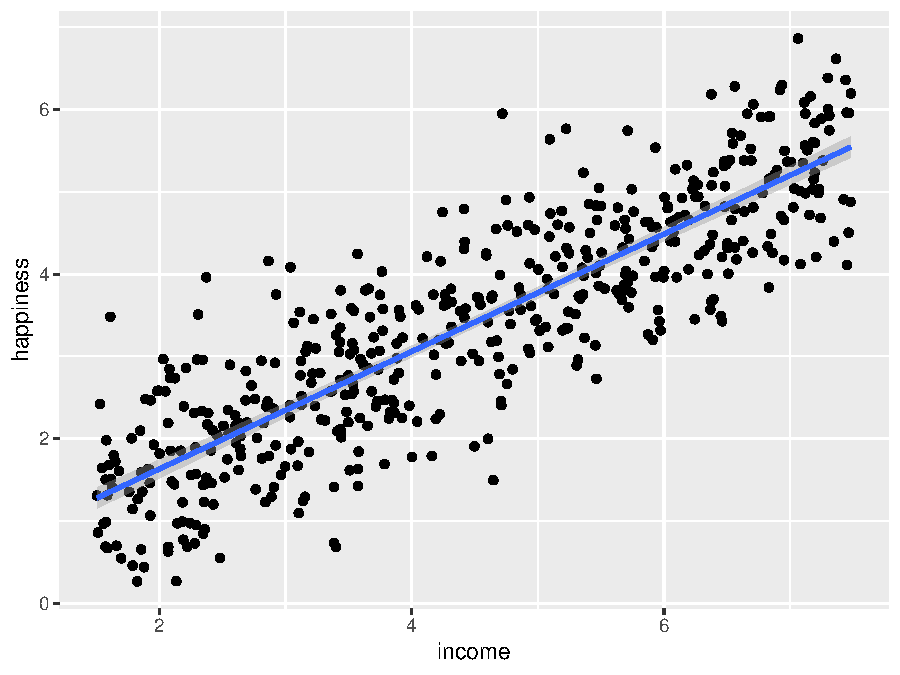
\includegraphics{03-simple-lm_files/figure-latex/lm1-1} 

}

\caption{La droite de régression}\label{fig:lm1}
\end{figure}

\hypertarget{graphes-des-ruxe9sidus}{%
\subsection{Graphes des résidus}\label{graphes-des-ruxe9sidus}}

On peut visualiser les résidus \(\hat\epsilon_i = y_i -\hat y_i\) afin de
voir leur dispersion autour de la moyenne \(0\). Les résidus peuvent être
obtenu dans le modèle entrainé \texttt{lm\_simple}, on y accède par
\texttt{\$residuals}.

\begin{Shaded}
\begin{Highlighting}[]
\NormalTok{X }\OtherTok{=}\NormalTok{ income}\SpecialCharTok{$}\NormalTok{income}
\NormalTok{residuals\_ }\OtherTok{=}\NormalTok{ lm\_simple}\SpecialCharTok{$}\NormalTok{residuals}
\FunctionTok{ggplot}\NormalTok{(}\AttributeTok{data =} \ConstantTok{NULL}\NormalTok{) }\SpecialCharTok{+} \FunctionTok{geom\_point}\NormalTok{(}\FunctionTok{aes}\NormalTok{(}\AttributeTok{x =}\NormalTok{ X,}\AttributeTok{y =}\NormalTok{residuals\_)) }\SpecialCharTok{+}
  \FunctionTok{geom\_abline}\NormalTok{(}\AttributeTok{slope =} \DecValTok{0}\NormalTok{, }\AttributeTok{intercept =} \DecValTok{0}\NormalTok{, }\AttributeTok{color =} \StringTok{\textquotesingle{}red\textquotesingle{}}\NormalTok{,}\AttributeTok{size =} \DecValTok{1}\NormalTok{)}
\end{Highlighting}
\end{Shaded}

\begin{figure}
\centering
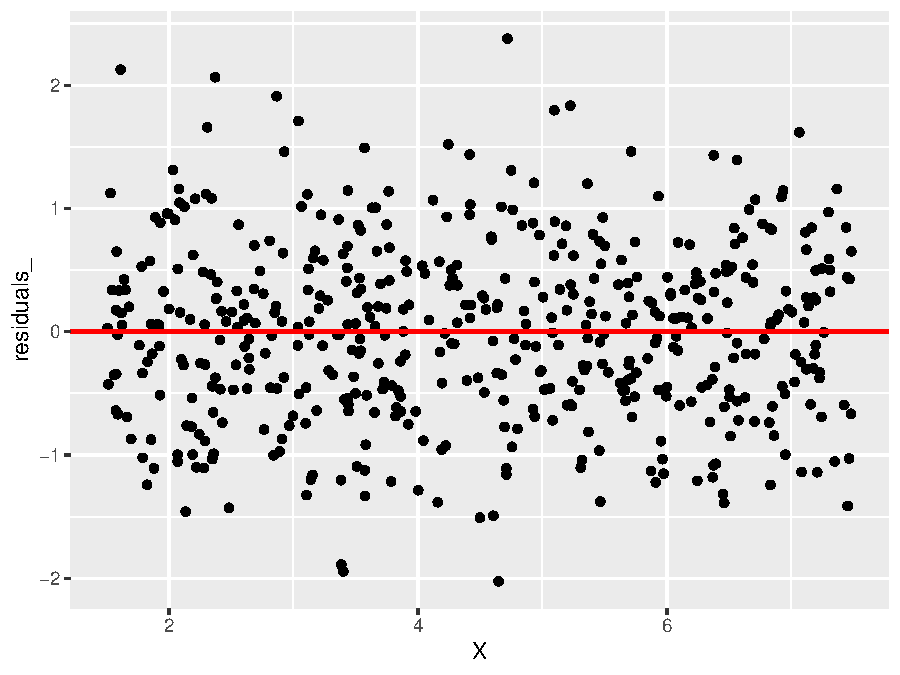
\includegraphics{03-simple-lm_files/figure-latex/unnamed-chunk-6-1.pdf}
\caption{\label{fig:unnamed-chunk-6}On voit bien que nos résidus se disperse de part et d'autre de 0}
\end{figure}

On peut aussi ajouter des sagements dans la figure \ref{fig:lm1} pour
visualiser les résidus. Nous allons choisir juste un échantillon de 50
observations.

\begin{Shaded}
\begin{Highlighting}[]
\CommentTok{\# Les indices choisis au hasard}
\NormalTok{echantillon }\OtherTok{=} \FunctionTok{sample}\NormalTok{(}\DecValTok{1}\SpecialCharTok{:}\DecValTok{498}\NormalTok{)[}\DecValTok{1}\SpecialCharTok{:}\DecValTok{50}\NormalTok{]}
\CommentTok{\# Echantillon des revenu}
\NormalTok{X\_residuals }\OtherTok{=}\NormalTok{ X[echantillon]}
\CommentTok{\# echention du niveau de bonheur}
\NormalTok{y }\OtherTok{=}\NormalTok{ income}\SpecialCharTok{$}\NormalTok{happiness[echantillon]}
\CommentTok{\# les y estimes correspondants a l\textquotesingle{}echantillon}
\NormalTok{y\_hat }\OtherTok{=}\NormalTok{ lm\_simple}\SpecialCharTok{$}\NormalTok{fitted.values[echantillon]}

\CommentTok{\# Representation de l\textquotesingle{}echantillon }
\FunctionTok{ggplot}\NormalTok{()}\SpecialCharTok{+} 
  \CommentTok{\# nuage de points}
  \FunctionTok{geom\_point}\NormalTok{(}\AttributeTok{data =}\NormalTok{ income,}\FunctionTok{aes}\NormalTok{(}\AttributeTok{x =}\NormalTok{income, }\AttributeTok{y =}\NormalTok{ happiness),}\AttributeTok{alpha =}\FloatTok{0.4}\NormalTok{) }\SpecialCharTok{+}
  \CommentTok{\# droite de regression}
  \FunctionTok{geom\_smooth}\NormalTok{(}\AttributeTok{data =}\NormalTok{ income,}\FunctionTok{aes}\NormalTok{(}\AttributeTok{x =}\NormalTok{income, }\AttributeTok{y =}\NormalTok{ happiness), }\AttributeTok{method =} \StringTok{\textquotesingle{}lm\textquotesingle{}}\NormalTok{) }\SpecialCharTok{+}
  \CommentTok{\# echantillon de y}
  \FunctionTok{geom\_point}\NormalTok{(}\FunctionTok{aes}\NormalTok{( }\AttributeTok{x=}\NormalTok{ X\_residuals, }\AttributeTok{y =}\NormalTok{ y), }\AttributeTok{color =}\StringTok{\textquotesingle{}red\textquotesingle{}}\NormalTok{, }\AttributeTok{size =} \DecValTok{2}\NormalTok{,) }\SpecialCharTok{+}
  \CommentTok{\#les erreurs}
  \FunctionTok{geom\_segment}\NormalTok{(}\FunctionTok{aes}\NormalTok{(}\AttributeTok{x =}\NormalTok{ X\_residuals, }\AttributeTok{y =}\NormalTok{ y\_hat, }\AttributeTok{xend =}\NormalTok{ X\_residuals, }\AttributeTok{yend =}\NormalTok{ y),}\AttributeTok{color =} \StringTok{\textquotesingle{}red\textquotesingle{}}\NormalTok{)}
\end{Highlighting}
\end{Shaded}

\begin{figure}
\centering
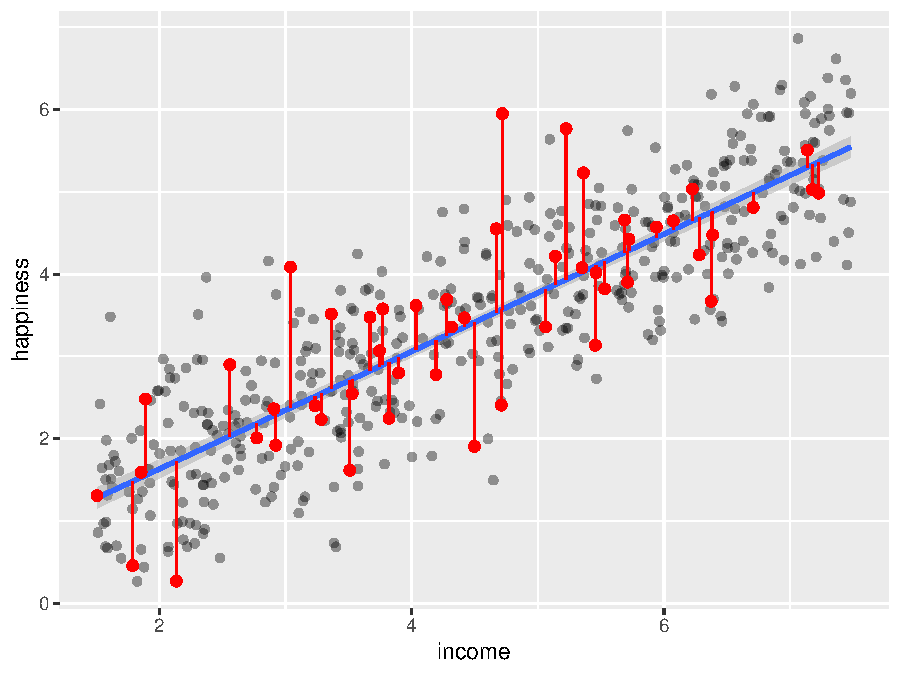
\includegraphics{03-simple-lm_files/figure-latex/residuals-1.pdf}
\caption{\label{fig:residuals}Les segments en rouges repressentent l'écart entre les valeurs estimées et les valeurs mesurées du niveau de bonheur (happiness)}
\end{figure}

\hypertarget{pruxe9diction}{%
\section{Prédiction}\label{pruxe9diction}}

Le but final d'une régression c'est de prédire des variables à
expliquées sans avoir à faire des mesures. Pour une nouvelle valeur de
\(X\) nous cherchons quel serait le \(y\) à partir de notre modèle.
Cette prédiction peut se faire sur R avec la fonction \texttt{predict()}.\\
On va reprendre notre modèle \texttt{lm\_simple} sauf que cette fois-ci, nous
n'allons pas entrainer un échantillon de \(100\) observations qui
représentent \(20\%\) de notre jeu de données \texttt{income}.

\begin{Shaded}
\begin{Highlighting}[]
\FunctionTok{set.seed}\NormalTok{(}\DecValTok{1234}\NormalTok{) }\CommentTok{\# pour fixer une racine a la fonction sample}
\NormalTok{echantillon }\OtherTok{=} \FunctionTok{sample}\NormalTok{(}\DecValTok{1}\SpecialCharTok{:}\DecValTok{498}\NormalTok{)[}\DecValTok{1}\SpecialCharTok{:}\DecValTok{100}\NormalTok{] }\CommentTok{\# indices de nos echantillons}
\NormalTok{data\_train }\OtherTok{=}\NormalTok{ income[}\SpecialCharTok{{-}}\NormalTok{echantillon,] }\CommentTok{\# data a entrainer}
\NormalTok{data\_test }\OtherTok{=}\NormalTok{ income[echantillon,] }\CommentTok{\# data non entrainé}
\NormalTok{lm\_simple }\OtherTok{=} \FunctionTok{lm}\NormalTok{(}\AttributeTok{data =}\NormalTok{ data\_train, }\AttributeTok{formula =}\NormalTok{ happiness}\SpecialCharTok{\textasciitilde{}}\NormalTok{income) }\CommentTok{\# entrainement du modele}
\end{Highlighting}
\end{Shaded}

\begin{Shaded}
\begin{Highlighting}[]
\CommentTok{\# prediction des y correspondants a notre echantillon de X}
\NormalTok{y\_predict }\OtherTok{=} \FunctionTok{predict}\NormalTok{(}\AttributeTok{object =}\NormalTok{ lm\_simple, }\AttributeTok{newdata =}\NormalTok{ data\_test[,}\DecValTok{1}\NormalTok{])}
\NormalTok{y\_predict[}\DecValTok{1}\SpecialCharTok{:}\DecValTok{10}\NormalTok{] }\CommentTok{\# Affichage des 10 premiers elements }
\CommentTok{\#\textgreater{}        1        2        3        4        5        6 }
\CommentTok{\#\textgreater{} 1.577312 5.114610 4.689354 4.817752 1.968143 1.504369 }
\CommentTok{\#\textgreater{}        7        8        9       10 }
\CommentTok{\#\textgreater{} 1.324728 3.422421 4.913247 3.493572}
\end{Highlighting}
\end{Shaded}

On peut visualiser la qualité de notre prédiction en représentant en
abscisse les \texttt{y\_test} et en ordonnée les \texttt{y\_predict}. Pour un modèle
parfait, le nuage de point doit être sur la première
bissectrice\footnote{la première bissectrice est une droite du plan muni d'un
  repère orthonormé, caractérisée par l'équation y = x}.

\begin{Shaded}
\begin{Highlighting}[]
\NormalTok{y\_test }\OtherTok{=}\NormalTok{ data\_test}\SpecialCharTok{$}\NormalTok{happiness}
\FunctionTok{ggplot}\NormalTok{() }\SpecialCharTok{+}
  \FunctionTok{geom\_point}\NormalTok{(}\FunctionTok{aes}\NormalTok{(}\AttributeTok{x =}\NormalTok{ y\_test, }\AttributeTok{y =}\NormalTok{ y\_predict)) }\SpecialCharTok{+}
  \FunctionTok{geom\_abline}\NormalTok{(}\AttributeTok{slope =} \DecValTok{1}\NormalTok{, }\AttributeTok{color =}\StringTok{\textquotesingle{}darkred\textquotesingle{}}\NormalTok{)  }\CommentTok{\# première bissectrice}
\end{Highlighting}
\end{Shaded}

\begin{figure}
\centering
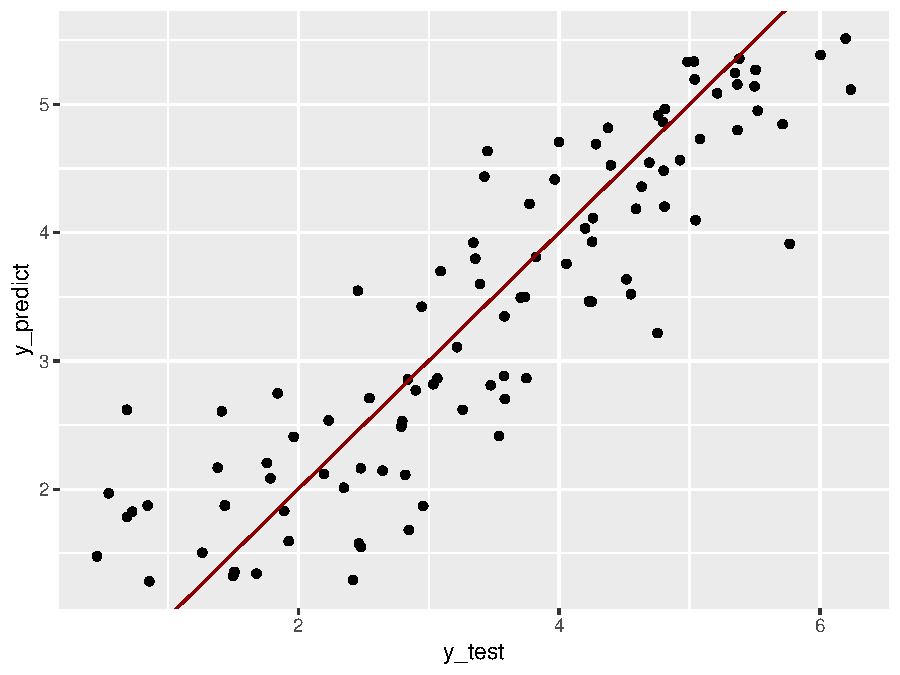
\includegraphics{03-simple-lm_files/figure-latex/unnamed-chunk-9-1.pdf}
\caption{\label{fig:unnamed-chunk-9}Représentations des y prédits en fonctions des y observés}
\end{figure}

Comme dans la figure\ref{fig:residuals}, nous pouvons représenter les
écarts entre les y prédits et les y observés sous forme de segments.

\begin{Shaded}
\begin{Highlighting}[]
\NormalTok{x\_test }\OtherTok{=}\NormalTok{ data\_test}\SpecialCharTok{$}\NormalTok{income}
\FunctionTok{ggplot}\NormalTok{() }\SpecialCharTok{+}
  \FunctionTok{geom\_point}\NormalTok{(}\AttributeTok{data =}\NormalTok{data\_test,}\FunctionTok{aes}\NormalTok{(income,happiness),}\AttributeTok{color =} \StringTok{\textquotesingle{}green\textquotesingle{}}\NormalTok{) }\SpecialCharTok{+}
  \FunctionTok{geom\_point}\NormalTok{(}\FunctionTok{aes}\NormalTok{(}\AttributeTok{x =}\NormalTok{ x\_test, }\AttributeTok{y =}\NormalTok{y\_predict), }\AttributeTok{color =}\StringTok{\textquotesingle{}blue\textquotesingle{}}\NormalTok{) }\SpecialCharTok{+}
  \FunctionTok{geom\_segment}\NormalTok{(}\FunctionTok{aes}\NormalTok{(}\AttributeTok{x =}\NormalTok{x\_test , }
                   \AttributeTok{y =}\NormalTok{ y\_test, }\AttributeTok{xend =}\NormalTok{ x\_test, }\AttributeTok{yend =}\NormalTok{ y\_predict),}\AttributeTok{color =} \StringTok{\textquotesingle{}red\textquotesingle{}}\NormalTok{)}
\end{Highlighting}
\end{Shaded}

\begin{figure}
\centering
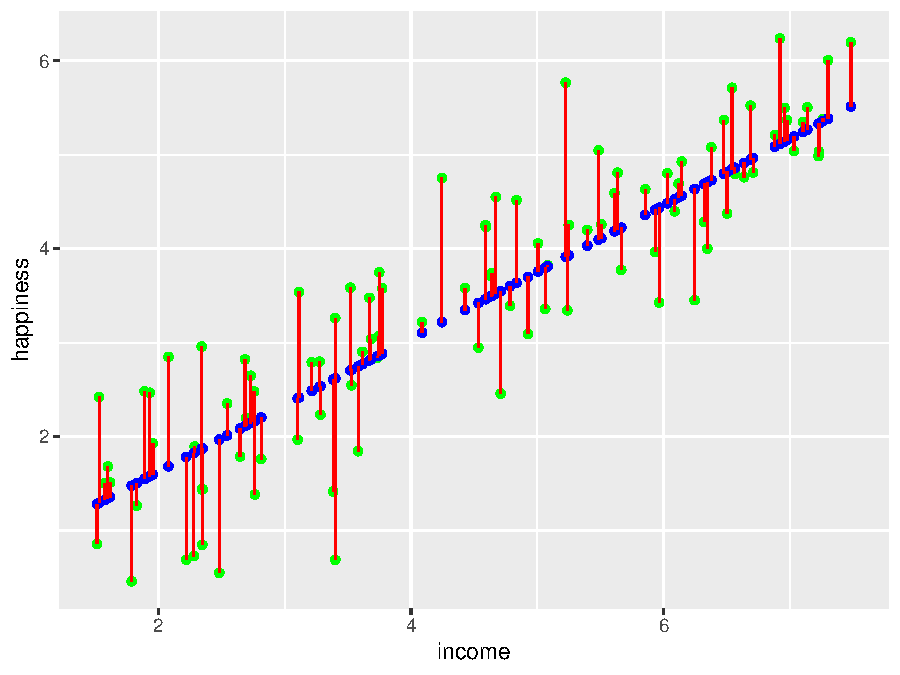
\includegraphics{03-simple-lm_files/figure-latex/unnamed-chunk-10-1.pdf}
\caption{\label{fig:unnamed-chunk-10}Les segments en rouges représentent les résidus, les points verts les y non entrainés qui ont servi au test et les points rouges représentent les y prédits à partir de notre modèle.}
\end{figure}

\hypertarget{ruxe9fuxe9rence}{%
\section*{Référence}\label{ruxe9fuxe9rence}}
\addcontentsline{toc}{section}{Référence}

\citet{lm_simple}

\hypertarget{multiple-lm}{%
\chapter{La régression linéaire multiple}\label{multiple-lm}}

Dans le chapitre précédent, nous avons cherché à expliquer une variable \(y\) par une seule variable quantitative \(X\) grâce à une fonction affine. Le modèle linéaire multiple est une généralisation du cas simple, en effet au lieu d'avoir une seule variable explicative nous en aurons plusieurs en nombre fini bien sûr, d'où le nom de régression lineaire multiple.
Les jeu de données \href{Data/heart.data.csv}{\texttt{heart\_data}} utilisé dans ce chapitre vient d'une enquête sur 500 villes, on a recueilli les données dans chaque ville en pourcentage de personnes atteintes de maladies cardiaques (\texttt{heart.disease}), qui fument(\texttt{smoking}) et qui se rendent au travail en vélo(\texttt{biking}). On cherche les facteurs qui pourraient avoir une influence sur les maladies cardiaques.

\begin{Shaded}
\begin{Highlighting}[]
\CommentTok{\# Load data}
\NormalTok{heart\_data }\OtherTok{\textless{}{-}} \FunctionTok{read.csv}\NormalTok{(}\StringTok{"Data/heart.data.csv"}\NormalTok{,}
                       \AttributeTok{header =}\NormalTok{ T,}\AttributeTok{sep =} \StringTok{","}\NormalTok{)}
\end{Highlighting}
\end{Shaded}

\hypertarget{moduxe9lisation-mathuxe9matique-1}{%
\section{Modélisation mathématique}\label{moduxe9lisation-mathuxe9matique-1}}

La relation affine dans le cas de la régression linéaire multiple est de la forme suivante :
\[y_i = \beta_0 + \beta_1x_{i1} + \beta_2x_{i2} +\dots+\beta_px_{ip}+\epsilon_{i}\;, \\ avec\;i\in\{1,2,3\dots,n\}\]

\begin{itemize}
\tightlist
\item
  \(y_i\) représentent la \(i\)ème valeur de la variable dépendantes \(y\).
\item
  \(x_{ij}\) représente la mesure de la \(i\)ème observation de la variable explicative \(X_j\)
\item
  les \(\beta_j\) sont les paramètres inconnus du modèle à estimer
\item
  \(\epsilon_i\) représente le bruit associé à la \(i\)ème observation\\
\end{itemize}

L'équation précédente peut être écrite sous une forme matricielle de cette manière :\\

\begin{equation}
y = X\beta +\epsilon
\label{eq:lm-multiple}
\end{equation}

avec :
\[ y = \begin{pmatrix}y_1\\y_2\\\vdots\\y_n \end{pmatrix} \hspace{.2cm} 
   X = \begin{pmatrix}
   1 & x_{11} & x_{12} & \dots &x_{1p}\\
   1 & x_{21} & x_{22} & \dots &x_{2p}\\
   \vdots &\vdots&\vdots & &\vdots\\
   1 & x_{n1} & x_{n2} & \dots &x_{np}
   \end{pmatrix} \hspace{.2cm}
   \beta = \begin{pmatrix}\beta_0\\\beta_1\\\vdots\\\beta_n \end{pmatrix} \hspace{.2cm}
   \epsilon = \begin{pmatrix}\epsilon_1\\\epsilon_2\\\vdots\\\epsilon_n \end{pmatrix} \hspace{.2cm}
\]

Dans notre jeu de données \texttt{heart\_data}, \(y\) représente le pourcentage de personnes atteintes de maladies cardiaques (\texttt{heart.disease}), \(X_1\) le pourcentage de personnes qui se rendent au travail en vélo(\texttt{biking}) et \(X_2\) le pourcentage de personnes qui fument(\texttt{smoking}).

\hypertarget{estimateurs-des-moindres-carruxe9s-ordinaires-mco}{%
\section{\texorpdfstring{Estimateurs des moindres carrés ordinaires (\(MCO\))}{Estimateurs des moindres carrés ordinaires (MCO)}}\label{estimateurs-des-moindres-carruxe9s-ordinaires-mco}}

Comme dans la régression linéaire simple, l'estimateur \(\hat\beta\) des moindres carrés de \(\beta\) est la quantité :\\

\[
\hat\beta =\operatorname*{argmin}_{(\beta_0,\beta_1\dots,\beta_p)}
\sum\limits_{i=1}^{n}{\Bigg(y_i - \sum\limits_{j=0}^{p}\beta_jx_{ij}\Bigg)}^2\\ 
= \operatorname*{argmin}_{\beta \in \mathbb{1}\times\mathbb{R}}\big(y-X\beta\big)'\big(y-X\beta\big) 
\]

La solution de cette équation est la suivante :~
\[
\hat\beta = (X'X)^{-1}(X'y)
\]\\
Une section entière dédiée au calcul de cet estimateur se trouve dans l'ouvrage \citet{lm_simple}.

\hypertarget{application-du-moduxe8le-linuxe9aire-multiple-avec-r}{%
\section{Application du modèle linéaire multiple avec R}\label{application-du-moduxe8le-linuxe9aire-multiple-avec-r}}

Le langage R permet d'entraîner le modèle linéaire multiple grâce à la fonction \texttt{lm()}. Pour indiquer à la fonction que nous sommes dans le cas d'une régression multiple, l'argument \texttt{formula} doit recevoir \texttt{y\textasciitilde{}X1+X2+...+XP} et pour notre exemple \texttt{heart.disease\textasciitilde{}biking+smoking}.
Lors qu'on précise l'argument data de la fonction lm et que les données ne contiennent que les variables à étudier, l'argument formel peut dans ce cas recevoir juste \texttt{y\textasciitilde{}.}. En Pratique, pour notre jeu de données \texttt{heart\_data}, ces deux écritures sont équivalentes :

\begin{Shaded}
\begin{Highlighting}[]
\NormalTok{lm\_multiple }\OtherTok{\textless{}{-}} \FunctionTok{lm}\NormalTok{(}\AttributeTok{formula =}\NormalTok{ heart.disease}\SpecialCharTok{\textasciitilde{}}\NormalTok{biking}\SpecialCharTok{+}\NormalTok{smoking, }\AttributeTok{data =}\NormalTok{ heart\_data)}
\NormalTok{lm\_multiple }\OtherTok{\textless{}{-}} \FunctionTok{lm}\NormalTok{(}\AttributeTok{formula =}\NormalTok{ heart.disease}\SpecialCharTok{\textasciitilde{}}\NormalTok{., }\AttributeTok{data =}\NormalTok{ heart\_data)}
\end{Highlighting}
\end{Shaded}

On peut afficher le résumé de l'entraînement de notre modèle avec la fonction \texttt{summary()}. Nous avons déjà appris la signification des éléments de la sortie de cette fonction dans la section\ref{OLS} du chapitre \ref{simple-lm}.

\begin{Shaded}
\begin{Highlighting}[]
\CommentTok{\# Resume du model}
\FunctionTok{summary}\NormalTok{(lm\_multiple)}
\CommentTok{\#\textgreater{} }
\CommentTok{\#\textgreater{} Call:}
\CommentTok{\#\textgreater{} lm(formula = heart.disease \textasciitilde{} ., data = heart\_data)}
\CommentTok{\#\textgreater{} }
\CommentTok{\#\textgreater{} Residuals:}
\CommentTok{\#\textgreater{}     Min      1Q  Median      3Q     Max }
\CommentTok{\#\textgreater{} {-}2.1789 {-}0.4463  0.0362  0.4422  1.9331 }
\CommentTok{\#\textgreater{} }
\CommentTok{\#\textgreater{} Coefficients:}
\CommentTok{\#\textgreater{}              Estimate Std. Error t value Pr(\textgreater{}|t|)    }
\CommentTok{\#\textgreater{} (Intercept) 14.984658   0.080137  186.99   \textless{}2e{-}16 ***}
\CommentTok{\#\textgreater{} biking      {-}0.200133   0.001366 {-}146.53   \textless{}2e{-}16 ***}
\CommentTok{\#\textgreater{} smoking      0.178334   0.003539   50.39   \textless{}2e{-}16 ***}
\CommentTok{\#\textgreater{} {-}{-}{-}}
\CommentTok{\#\textgreater{} Signif. codes:  }
\CommentTok{\#\textgreater{} 0 \textquotesingle{}***\textquotesingle{} 0.001 \textquotesingle{}**\textquotesingle{} 0.01 \textquotesingle{}*\textquotesingle{} 0.05 \textquotesingle{}.\textquotesingle{} 0.1 \textquotesingle{} \textquotesingle{} 1}
\CommentTok{\#\textgreater{} }
\CommentTok{\#\textgreater{} Residual standard error: 0.654 on 495 degrees of freedom}
\CommentTok{\#\textgreater{} Multiple R{-}squared:  0.9796, Adjusted R{-}squared:  0.9795 }
\CommentTok{\#\textgreater{} F{-}statistic: 1.19e+04 on 2 and 495 DF,  p{-}value: \textless{} 2.2e{-}16}
\end{Highlighting}
\end{Shaded}

On constate que pour toutes les variables y compris l'Intercept, les p-values sonts très inférieures à \(5\%\), on rejette alors l'hypothèse \(H_0\) insinuant que \(\beta_j\) est nulle avec un niveau de confiance de \(95\%\).\\
De plus, le coefficient d'ajustement \(R^2\) est de \(0.9796\), soit un score de \(97,96\%\) pour notre modèle ce qui est un très bon résultat.

Lors de la régression multiple, on peut s'intéresser à l'effet de l'interaction entre les variables explicatives sur la variable \(y\). L'étude de cette interaction peut se faire dans notre exemple par la \texttt{formula} \texttt{heart.disease\textasciitilde{}biking+smoking+biking:smoking} où la troisième composante \texttt{biking:smoking} représente l'interaction entre le pourcentage de personnes qui se rendent au travail en vélo et le pourcentage de personnes qui fument. Cette écriture peut prendre une forme plus simple telle que \texttt{heart.disease\textasciitilde{}biking*smoking}. \texttt{lm\_multiple} devient alors :

\begin{Shaded}
\begin{Highlighting}[]
\NormalTok{lm\_multiple }\OtherTok{\textless{}{-}} \FunctionTok{lm}\NormalTok{(}\AttributeTok{formula =}\NormalTok{ heart.disease}\SpecialCharTok{\textasciitilde{}}\NormalTok{biking}\SpecialCharTok{*}\NormalTok{smoking, }\AttributeTok{data =}\NormalTok{ heart\_data)}
\FunctionTok{summary}\NormalTok{(lm\_multiple)}
\CommentTok{\#\textgreater{} }
\CommentTok{\#\textgreater{} Call:}
\CommentTok{\#\textgreater{} lm(formula = heart.disease \textasciitilde{} biking * smoking, data = heart\_data)}
\CommentTok{\#\textgreater{} }
\CommentTok{\#\textgreater{} Residuals:}
\CommentTok{\#\textgreater{}      Min       1Q   Median       3Q      Max }
\CommentTok{\#\textgreater{} {-}2.20619 {-}0.44862  0.02892  0.44099  1.94142 }
\CommentTok{\#\textgreater{} }
\CommentTok{\#\textgreater{} Coefficients:}
\CommentTok{\#\textgreater{}                  Estimate Std. Error t value Pr(\textgreater{}|t|)    }
\CommentTok{\#\textgreater{} (Intercept)    15.0527397  0.1248112 120.604   \textless{}2e{-}16 ***}
\CommentTok{\#\textgreater{} biking         {-}0.2019916  0.0029472 {-}68.536   \textless{}2e{-}16 ***}
\CommentTok{\#\textgreater{} smoking         0.1740065  0.0070359  24.731   \textless{}2e{-}16 ***}
\CommentTok{\#\textgreater{} biking:smoking  0.0001177  0.0001653   0.712    0.477    }
\CommentTok{\#\textgreater{} {-}{-}{-}}
\CommentTok{\#\textgreater{} Signif. codes:  }
\CommentTok{\#\textgreater{} 0 \textquotesingle{}***\textquotesingle{} 0.001 \textquotesingle{}**\textquotesingle{} 0.01 \textquotesingle{}*\textquotesingle{} 0.05 \textquotesingle{}.\textquotesingle{} 0.1 \textquotesingle{} \textquotesingle{} 1}
\CommentTok{\#\textgreater{} }
\CommentTok{\#\textgreater{} Residual standard error: 0.6544 on 494 degrees of freedom}
\CommentTok{\#\textgreater{} Multiple R{-}squared:  0.9796, Adjusted R{-}squared:  0.9795 }
\CommentTok{\#\textgreater{} F{-}statistic:  7922 on 3 and 494 DF,  p{-}value: \textless{} 2.2e{-}16}
\end{Highlighting}
\end{Shaded}

Dans la nouvelle sortie on peut voir une nouvelle variable \texttt{biking:smoking} dont la p-value est très proche de \(5\%\) donc par prudence, on ne peut rejeter l'hypothèse nulle \(H_0\) associée au \(\beta_j\) de cette variable. Autrement dit, on peut se passer de l'interaction entre \texttt{biking}(\(X_1\)) et \texttt{smoking}(\(X_2\)) dans l'explication de \texttt{heart.disease}(\(y\)).

\hypertarget{repruxe9sentations-graphiques-1}{%
\section{Représentations graphiques}\label{repruxe9sentations-graphiques-1}}

Lorsque le nombre de variables explicatives dépasse 2, il est impossible de représenter sur un même graphes le nuage de point formé par y, en effet la dimension physique maximale est de 3.
Il existe plusieurs packages qui donnes des représentations assez significatives en deux dimensions du modèle lineair multiple tel que \texttt{car}\footnote{package car : \url{https://cran.r-project.org/web/packages/car/index.html}}.

\hypertarget{nuage-de-points-3d}{%
\subsection{Nuage de points 3D}\label{nuage-de-points-3d}}

Pour notre exemple nous pouvons faire une représentation interactive en 3 dimensions de nos variable avec la fonction \texttt{plot\_ly()} du package \texttt{plotly}.

\begin{Shaded}
\begin{Highlighting}[]
\FunctionTok{library}\NormalTok{(plotly)}
\NormalTok{figure }\OtherTok{\textless{}{-}} \FunctionTok{plot\_ly}\NormalTok{(heart\_data, }\AttributeTok{x =} \SpecialCharTok{\textasciitilde{}}\NormalTok{biking, }\AttributeTok{y =} \SpecialCharTok{\textasciitilde{}}\NormalTok{smoking, }\AttributeTok{z =} \SpecialCharTok{\textasciitilde{}}\NormalTok{heart.disease, }
   \AttributeTok{color =}\SpecialCharTok{\textasciitilde{}}\NormalTok{heart.disease}
\NormalTok{  ) }\SpecialCharTok{\%\textgreater{}\%}
  \FunctionTok{add\_markers}\NormalTok{() }\SpecialCharTok{\%\textgreater{}\%}
  \FunctionTok{layout}\NormalTok{(}
    \AttributeTok{scene =} \FunctionTok{list}\NormalTok{(}\AttributeTok{xaxis =} \FunctionTok{list}\NormalTok{(}\AttributeTok{title =} \StringTok{\textquotesingle{}biking\textquotesingle{}}\NormalTok{),}
        \AttributeTok{yaxis =} \FunctionTok{list}\NormalTok{(}\AttributeTok{title =} \StringTok{\textquotesingle{}smoking\textquotesingle{}}\NormalTok{),}
        \AttributeTok{zaxis =} \FunctionTok{list}\NormalTok{(}\AttributeTok{title =} \StringTok{\textquotesingle{}heart.disease\textquotesingle{}}\NormalTok{))}
\NormalTok{        )}
\NormalTok{figure}
\end{Highlighting}
\end{Shaded}

\begin{figure}
\centering

\includegraphics{04-multiple-lm_files/figure-latex/nuage3d-1.pdf}
\caption{\label{fig:nuage3d}Nuage de points en 3D}
\end{figure}

Une représentation 3 dimensions plus simple peut être faite avec la fonction \texttt{scatterplot3d()} du package de même nom.

\begin{Shaded}
\begin{Highlighting}[]
\FunctionTok{library}\NormalTok{(scatterplot3d)}
\FunctionTok{scatterplot3d}\NormalTok{(}\AttributeTok{x =}\NormalTok{heart\_data[,}\StringTok{"biking"}\NormalTok{],}
                         \AttributeTok{y =}\NormalTok{ heart\_data[,}\StringTok{"smoking"}\NormalTok{],}
                         \AttributeTok{z=}\NormalTok{ heart\_data[,}\StringTok{"heart.disease"}\NormalTok{], }\AttributeTok{type=}\StringTok{"p"}\NormalTok{,}\AttributeTok{pch=}\DecValTok{16}\NormalTok{,}\AttributeTok{box=}\ConstantTok{FALSE}\NormalTok{,}
                         \AttributeTok{xlab=}\StringTok{"biking"}\NormalTok{,}\AttributeTok{ylab=}\StringTok{"smoking"}\NormalTok{,}\AttributeTok{zlab=}\StringTok{"heart.disease"}\NormalTok{)}
\end{Highlighting}
\end{Shaded}

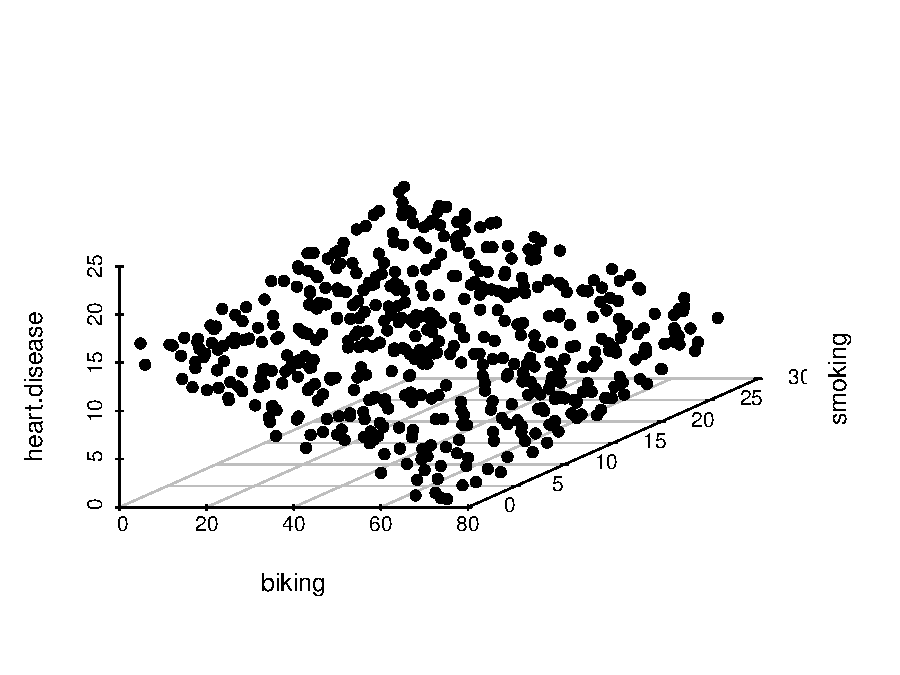
\includegraphics{04-multiple-lm_files/figure-latex/unnamed-chunk-5-1.pdf}

\hypertarget{droite-de-ruxe9gression}{%
\subsection{Droite de régression}\label{droite-de-ruxe9gression}}

La représentation de la droite de régression peut se faire sur chaque dimension des variables explicative grâce à la fonction \texttt{avPlots()} de la libraire car

\begin{Shaded}
\begin{Highlighting}[]
\FunctionTok{library}\NormalTok{(car)}
\FunctionTok{avPlots}\NormalTok{(lm\_multiple)}
\end{Highlighting}
\end{Shaded}

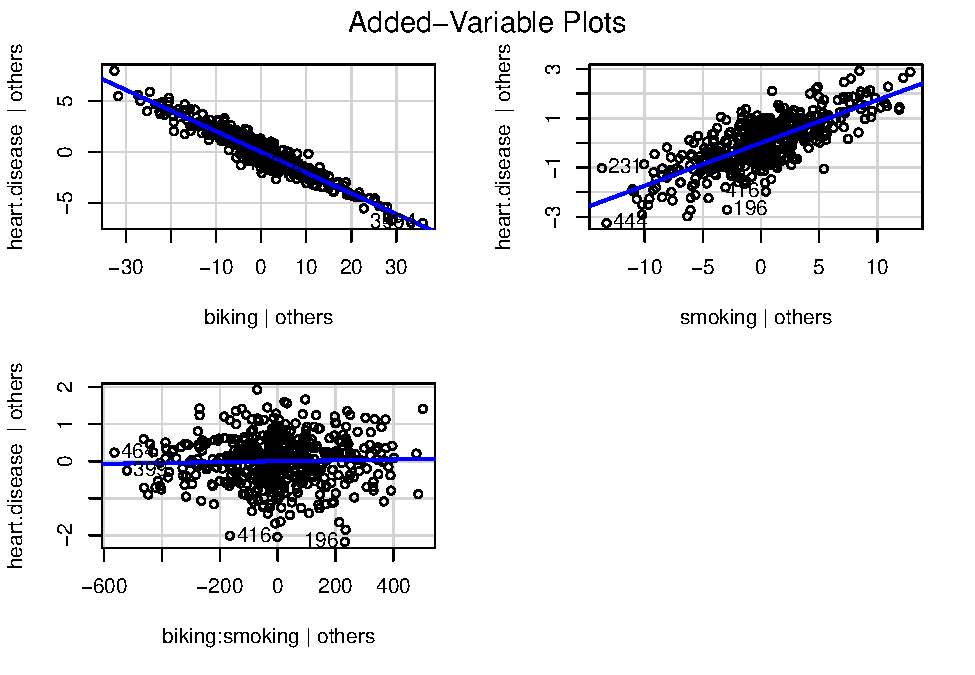
\includegraphics{04-multiple-lm_files/figure-latex/lm_multiple-1.pdf}
\#\# Prédiction
La prédiction dans le modèle linéaire multiple se fait aussi avec la fonction \texttt{predict()} comme dans le cas simple. On peut reprendre l'entraînement de notre modèle avec \(80\%\) de nos données soient 400 observations et utiliser les \(20\%\) pour effectuer une prédiction. Cela peut nous permettre de voir les résidus entre les valeurs prédites et les valeurs réelles de \(y\).

\begin{Shaded}
\begin{Highlighting}[]
\FunctionTok{set.seed}\NormalTok{(}\DecValTok{2345}\NormalTok{)}
\NormalTok{echantillon }\OtherTok{=} \FunctionTok{sample}\NormalTok{(}\DecValTok{1}\SpecialCharTok{:}\DecValTok{498}\NormalTok{)[}\DecValTok{1}\SpecialCharTok{:}\DecValTok{100}\NormalTok{]}
\NormalTok{data\_train }\OtherTok{\textless{}{-}}\NormalTok{ heart\_data[}\SpecialCharTok{{-}}\NormalTok{echantillon,]}
\NormalTok{data\_test }\OtherTok{\textless{}{-}}\NormalTok{ heart\_data[echantillon,]}
\NormalTok{model }\OtherTok{\textless{}{-}} \FunctionTok{lm}\NormalTok{(heart.disease}\SpecialCharTok{\textasciitilde{}}\NormalTok{.,}\AttributeTok{data =}\NormalTok{ data\_test)}
\CommentTok{\# Prediction}
\NormalTok{y\_predict }\OtherTok{\textless{}{-}} \FunctionTok{predict}\NormalTok{(model,data\_test[,}\SpecialCharTok{{-}}\DecValTok{3}\NormalTok{])}
\NormalTok{y\_predict[}\DecValTok{1}\SpecialCharTok{:}\DecValTok{10}\NormalTok{]}
\CommentTok{\#\textgreater{}       483       494       359       211       418       335 }
\CommentTok{\#\textgreater{} 10.222660 10.432554 13.843535 16.974577  6.824394 12.325991 }
\CommentTok{\#\textgreater{}       204       475        67        66 }
\CommentTok{\#\textgreater{}  5.947508 12.011159 12.926691 18.413173}
\end{Highlighting}
\end{Shaded}

On peut visualiser les résidus entre les variables \(y_i\) observés et les \(y_i\) prédites :

\begin{Shaded}
\begin{Highlighting}[]
\FunctionTok{library}\NormalTok{(ggplot2)}
\NormalTok{y\_test }\OtherTok{=}\NormalTok{ data\_test}\SpecialCharTok{$}\NormalTok{heart.disease}
\FunctionTok{ggplot}\NormalTok{() }\SpecialCharTok{+}
  \FunctionTok{geom\_point}\NormalTok{(}\FunctionTok{aes}\NormalTok{(}\AttributeTok{x =}\NormalTok{ y\_test, }\AttributeTok{y =}\NormalTok{ y\_predict)) }\SpecialCharTok{+}
  \FunctionTok{geom\_abline}\NormalTok{(}\AttributeTok{slope =} \DecValTok{1}\NormalTok{, }\AttributeTok{color =}\StringTok{\textquotesingle{}darkred\textquotesingle{}}\NormalTok{) }\SpecialCharTok{+}
  \FunctionTok{geom\_segment}\NormalTok{(}\FunctionTok{aes}\NormalTok{(}\AttributeTok{x =}\NormalTok{y\_test , }
                   \AttributeTok{y =}\NormalTok{ y\_test, }\AttributeTok{xend =}\NormalTok{ y\_test, }\AttributeTok{yend =}\NormalTok{ y\_predict),}
               \AttributeTok{color =} \StringTok{\textquotesingle{}red\textquotesingle{}}\NormalTok{) }\SpecialCharTok{+}
  \FunctionTok{ylab}\NormalTok{(}\StringTok{"Predicted heart disease"}\NormalTok{)}\SpecialCharTok{+}\FunctionTok{xlab}\NormalTok{(}\StringTok{"Heart disease"}\NormalTok{)}
\end{Highlighting}
\end{Shaded}

\begin{figure}
\centering
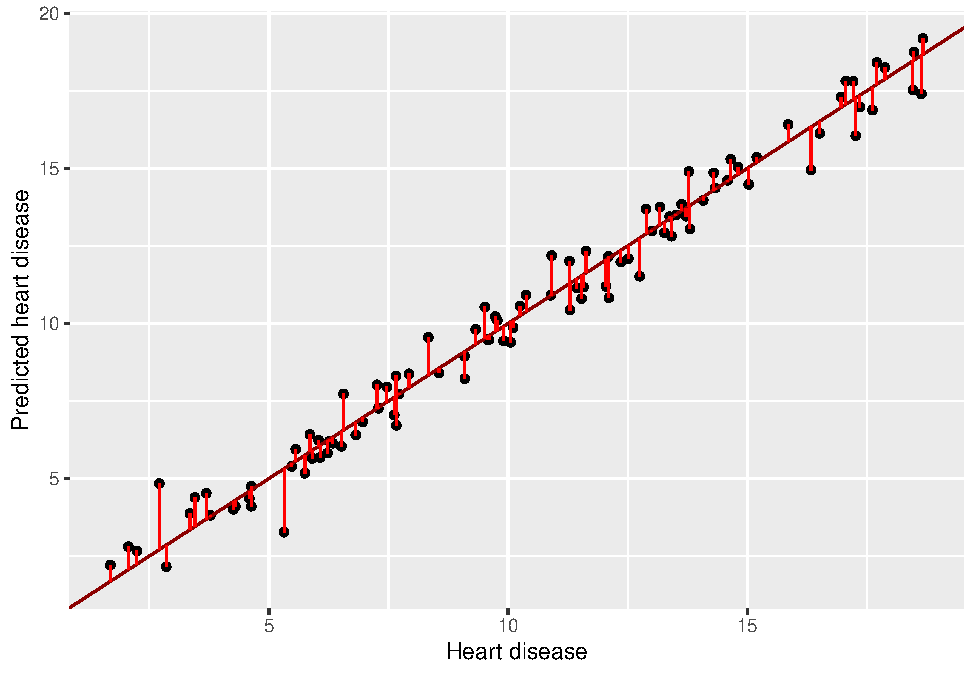
\includegraphics{04-multiple-lm_files/figure-latex/unnamed-chunk-7-1.pdf}
\caption{\label{fig:unnamed-chunk-7}Les résidus sont très proches de 0 cela qui reflète la bonne qualité du modèle.}
\end{figure}

\hypertarget{glm}{%
\chapter{Le modèle linéaire généralisé}\label{glm}}

\hypertarget{anova1}{%
\chapter{Analyse de la variance à un facteur}\label{anova1}}

\hypertarget{anova2}{%
\chapter{Analyse de la variance à deux facteurs}\label{anova2}}

\hypertarget{ancova}{%
\chapter{Analyse de la covariance}\label{ancova}}

\hypertarget{part-iii-suxe9ries-chronologiques}{%
\part{III-Séries chronologiques}\label{part-iii-suxe9ries-chronologiques}}

\hypertarget{intro-ts}{%
\chapter{Introduction}\label{intro-ts}}

\hypertarget{duxe9finition-5}{%
\section{Définition}\label{duxe9finition-5}}

\hypertarget{exemples}{%
\section{Exemples}\label{exemples}}

\hypertarget{tendances-et-saisonnalituxe9s}{%
\chapter{Tendances et saisonnalités}\label{tendances-et-saisonnalituxe9s}}

\hypertarget{processus-stationnaire}{%
\section{Processus stationnaire}\label{processus-stationnaire}}

\hypertarget{estimation-paramuxe9trique-de-la-tendance}{%
\section{Estimation paramétrique de la tendance}\label{estimation-paramuxe9trique-de-la-tendance}}

\hypertarget{estimation-non-paramuxe9trique}{%
\section{Estimation non paramétrique}\label{estimation-non-paramuxe9trique}}

\hypertarget{elimination-du-trend-et-de-la-saisonnalituxe9}{%
\section{Elimination du trend et de la saisonnalité}\label{elimination-du-trend-et-de-la-saisonnalituxe9}}

\hypertarget{series-stat}{%
\chapter{Séries stationnaires}\label{series-stat}}

\hypertarget{processus-linuxe9aires-et-processus-linuxe9aires-guxe9nuxe9raux}{%
\section{Processus linéaires et processus linéaires généraux}\label{processus-linuxe9aires-et-processus-linuxe9aires-guxe9nuxe9raux}}

\hypertarget{les-processus-armapq}{%
\section{Les processus ARMA(p,q)}\label{les-processus-armapq}}

\hypertarget{processusmaq}{%
\subsection{ProcessusMA(q)}\label{processusmaq}}

\hypertarget{processus-arp}{%
\subsection{Processus AR(p)}\label{processus-arp}}

\hypertarget{autocovariance-des-processus-arma}{%
\section{Autocovariance des processus ARMA}\label{autocovariance-des-processus-arma}}

\hypertarget{proc-non-stat}{%
\chapter{Séries non stationnaires}\label{proc-non-stat}}

\hypertarget{processus-arima}{%
\section{Processus ARIMA}\label{processus-arima}}

\hypertarget{processus-sarima}{%
\section{Processus SARIMA}\label{processus-sarima}}

\hypertarget{ARCH-GARCH}{%
\chapter{Processus ARCH et GARCH}\label{ARCH-GARCH}}

\hypertarget{duxe9finition-6}{%
\section{Définition}\label{duxe9finition-6}}

\hypertarget{moduxe8les-arch}{%
\section{Modèles ARCH}\label{moduxe8les-arch}}

\hypertarget{moduxe8les-garch}{%
\section{Modèles GARCH}\label{moduxe8les-garch}}

\hypertarget{moduxe8lesarma-garch}{%
\section{ModèlesARMA-GARCH}\label{moduxe8lesarma-garch}}

  \bibliography{book.bib,packages.bib}

\end{document}
